\documentclass[12pt]{article}
\sloppy %prevent text overflowing margins

\usepackage{amsmath}
\usepackage{amssymb}
\usepackage{array}
\usepackage{graphicx}
\usepackage{mathtools}
\usepackage{subcaption}
\usepackage{float}
\usepackage[none]{hyphenat} %prevent hypenation
\usepackage[margin=2.5cm]{geometry}
\renewcommand{\baselinestretch}{1.5}
\usepackage[square]{natbib}
\usepackage{setspace}
\usepackage{sidecap}
\usepackage{tablefootnote}
\usepackage{makecell}

\graphicspath{{Graphs/}{Images/}}
\DeclarePairedDelimiter{\ceil}{\lceil}{\rceil}

\usepackage{CJKutf8} %Japanese
\DeclareUnicodeCharacter{202D}{}
\DeclareUnicodeCharacter{202C}{}
\DeclareUnicodeCharacter{3000}{}

\usepackage{minted}
%Setting number size
\renewcommand\theFancyVerbLine{\normalsize\arabic{FancyVerbLine}}

\usepackage{listings}

\usepackage{fancyhdr}
\pagestyle{fancy}
\lhead{Lewis Wilson}
\chead{Practical Lossless Data Compression}
\rhead{1413099/ma14ljw}

%tree diagrams
\usepackage{tikz}
\usepackage{tikz-qtree}

\onehalfspacing %sets line spacing to 1.5

\title{Practical Lossless Data Compression}
\author{\textbf{Lewis Wilson} \\
	BSc Mathematics with Computer Science\\\\
	Department of Mathematics, College of Engineering,\\ 
	Design and Physical Sciences, Brunel University.\\\\
	Supervisor: Dr. Aleksey Pichugin}
\date{Year of Submission: 2017/2018}

\begin{document}
	
\begin{titlepage}
\maketitle
\thispagestyle{empty} %Removes page number
\begin{figure}[b!]
	\centering
	
\includegraphics[width=3.5in]{brunel_logo}
\end{figure}
\end{titlepage}

\pagenumbering{roman}
\setcounter{tocdepth}{2}
\tableofcontents

\clearpage
\listoffigures

\clearpage
\listoftables
\newpage

\section*{Acknowledgements}

I would like to take this opportunity to show my appreciation to numerous individuals who have aided and supported me during the course of this project. This thanks is largely projected towards my dissertation supervisor Dr. Aleksey Pichugin for providing me with a wealth of technical support. It is thanks to Dr. Pichugin, and his guidance that this dissertation has been possible.

Additionally, I would like to thank all of my current and previous lecturers from both the Mathematics and Computer Science departments at Brunel University London for their contribution to my technical and mathematical understanding of topics presented in this dissertation.

Finally, I extend my appreciation to my family who have always motivated me to succeed academically. They have provided me moral support and advice throughout my time at University and during the course of this project, for which I am extremely grateful.

\clearpage

\begin{abstract}
This paper discusses lossless data compression and why it is important; it includes reference information for fixed and variable-length code techniques, as well as for the Huffman Coding, Lempel-Ziv-77 (LZ77) and Lempel-Ziv-4 (LZ4) data compression methods. Huffman Coding and LZ77 provide the basis for many lossless compression techniques currently in use today, while LZ4 builds upon the ideas presented in LZ77.

The focus of this research is solely on lossless data compression, rather than lossy compression. Lossy compression is used in a variety of file formats, such as JPEG, PNG and MP3, however the original data set is reduced, hence this is out of scope.

Contained within this document are details of implementations of a Huffman Encoder and Decoder and a LZ4 Encoder and Decoder, written in the `Octave' programming language. Each compressor implemented successfully compresses a set of 13 test files with varying average compression values. While implementations are included generally, the specifics can (often) be altered, dependent on any specifications in place. Due to the generalisations presented, each implementation can be written in any desired programming language.

On analysing the compression results of the included implementations, these are compared to popular commercial and open-source compressors available online, namely smalLZ4 (an optimal LZ4 compressor), WinRAR (popular with Microsoft Windows users) and 7-Zip (known for its high average compression rates). Overall, it is found that the LZ4 implementation can be configured to compress the 13 test files considerably more than the Huffman implementation. One downside of this configuration is that the runtime for LZ4 can be much slower than that of Huffman, however if time is no object, the LZ4 implementation presented can definitely produce more impressive compression results. With this in mind, the Huffman and LZ4 encoders cannot compete with the likes of WinRAR and 7-Zip, in fact as smalLZ4 is optimal LZ4 encoding, the LZ4 implementation alone will be unable to perform as well WinRAR or 7-Zip on the included test files in terms of compression. This does guarantee that a merging of multiple compression techniques would be ineffective however.
\end{abstract}

\clearpage

\setcounter{page}{1} %begin from page 1 here
\pagenumbering{arabic}

\section{Introduction}
\subsection{Prerequisites}
To become familiar with practical data compression, it is essential to have:

\begin{itemize}
	\item An understanding of computer data structures, hexadecimal systems, raw data and how binary operations are performed;
	\item Basic knowledge of algorithms regarding how they function and how they are interpreted by computers;
	\item An idea of how digital storage works and how efficiency is calculated;
	\item An understanding of mathematical fundamentals including sets, matrix computation, simple trigonometry and basic probability theory \citep{ipu_dc}.
\end{itemize}

\begin{flushleft}
	Supplementary to these prerequisites, it would be helpful to have the following skills:
\end{flushleft}

\begin{itemize}
	\item A knowledge of encoding schemes such as the American Standard Code for Information Interchange 8 (ASCII-8) and Unicode, to be able to understand how bytes are converted into characters;
	\item Understanding of programming languages and their syntaxes; preferably Matlab or Octave, as implementations will be written in Octave.
\end{itemize}

\subsection{Background}
Compression is essential in the age of computers as data is consistently created and rarely deleted. With this trend in data creation, both the requirements for an increase in storage capacity and efficiency of data compression have become important.

In general, the term `compression' refers to reducing the overall volume or size of something. Applying this definition to computing, `compression' (or `data compression') refers to the reduction in size of a piece (or pieces) of data on a hard-drive or other storage medium.

General computer users are often, and possibly obliviously, subject to data compression. `Zipped' (ZIP) and `Roshal Archive' (RAR) files commonly act as compressed containers to store many/large data items where `Joint Photographic Experts Group' (JPEG) compression is used to reduce the file size of photographs and other images. Behind compressed file types are specific methods to achieving their compression, including Huffman Coding and Lempel-Ziv-77 (LZ77), which are to be discussed later on in this paper.

Additionally to saving storage space for users locally on their computers, compression via the public internet is very important. Many services on the internet enable users to access large portions of data in almost real-time. One such example of these services is Netflix for streaming audio and video data. Without data compression applied to files, streaming services would be far less efficient for both hosts and clients; raw video consumes a vast amount of bandwidth, therefore using compression helps to achieve respectable transmission efficiency \citep{internet_video_streaming}. 

There are two types of data compression, lossless and lossy. Lossless compression provides a reduction in the size of data without the loss of any content after decompression (e.g. ZIP), whereas lossy compression conversely removes any seemingly unnecessary articles from the data, thus reducing its size (e.g. JPEG).

There are many different algorithmic approaches to compression. For lossless compression particularly, the methodologies can be classified as symbol-based and dictionary-based. As examples, Huffman Coding provides a symbol-based method of approach using variable code lengths, whereas LZ77 is dictionary-based \citep{dc_complete_ref}. It is not uncommon for a combination of approaches to be applied. Taking DEFLATE as an example algorithm, this uses a combination of LZ77 and Huffman Coding to achieve good compression. For DEFLATE, this compression level can be altered depending on if time or compression ratio is most important \citep{deflate_rfc}.

One issue in the domain of compression are the speeds at which compression and decompression are completed. Often there is a trade-off between the compression levels and the compression/decompression speeds \citep[p.~5]{dc_complete_ref}. Different algorithms tend to have their own unique solution to addressing this issue. 


\subsection{Motivation}
Having had an interest in computers for a number of years and studying Mathematics with Computer Science, I was drawn to a project involving a combination of both subjects. During my placement year, I had an informal conversation with a colleague about data compression and the underlying techniques. Since then, I have been fascinated by the idea storing large amounts of data in smaller spaces, whilst maintaining a complete set of data.

Additionally, whilst this is a topic of interest to me, I also believe it is an important one that benefits many computer users on a daily basis. Without data compression, there could be a number of complications such as extended loading times and a potential for the impossibility of data streaming.

To supplement my learning, I have also chosen to take the Mathematics module MA3236: Data Compression and Encryption. In this module, theory of Huffman Coding is taught. While encryption can be applied during compression of data, it is out of scope for this project.

\subsection{Applications}
There are many lossless compression algorithms that have practical implementations. Some such example algorithms include \citep[p.~1050-1065]{dc_complete_ref}:

\begin{itemize}
	\item \textbf{Huffman Coding}: a method of lossless compression used in a variety of popular computer programs;
	
	\item \textbf{LZ77}: a dictionary based method used as the basis of many other dictionary compression methods. LZ77 and its variants are used in reducing text, image and audio file sizes;
	
	\item \textbf{DEFLATE}: an algorithm that combines the Huffman Coding and LZ77 methods. This is used for compression of files into a ZIP file container \citep{deflate_rfc};
	
	\item \textbf{RAR}: Popular with Windows users, has options for error-correcting and encrypting stored data. RAR was initially a variant of LZ77, however has been thoroughly developed since its initial release;
	
	\item \textbf{Free Lossless Audio Compression (FLAC)}: used to compress audio files while maintaining their quality.
	
\end{itemize}

\subsection{Dissertation Focus}
This paper will focus primarily on methods of lossless compression rather than the lossy type. The two main approaches of compression to be considered will be Huffman Coding, a symbol-based technique and Lempel-Ziv-4 (LZ4), a dictionary-based technique whilst also considering how LZ4 derives from LZ77. 

I shall be programming my own implementations of an encoder and a decoder for both Huffman Coding and LZ4. These implementations will be produced using Octave which is a free tool used for programming in a MatLab-style syntax. I have chosen Octave as this language has many useful functions and tools that I can utilise for mathematical and algorithmic implementation of Huffman Coding and LZ4. Something else to note, is that I have found very minimal documentation of Huffman Coding and LZ4 being successfully implemented in Octave; regarding this, I have made sure to challenge my programming strengths and weaknesses.

\subsection{Objectives}{\label{sec_objectives}}
I have set myself four main objectives for the course of this project, these are:

\begin{enumerate}
	\item \textbf{Produce two working data compressors}: As a minimum, two data compression algorithms will be implemented, one symbol-based and one dictionary-based;
	
	\item \textbf{Achieve a good level of compression}: Each algorithm produced should achieve a good level of compression. I have estimated that the average compression will be approximately 70\% of the size of the original file;
	
	\item \textbf{Understand the suitability of algorithm types}: Become aware of the advantages and disadvantages of different types of algorithm. E.g. Are there certain types of data in which symbol-based methods are desired over dictionary-based methods?;
	
	\item \textbf{Deliver a high-quality, detailed dissertation write-up}: This should include how the research is useful and how it aligns to practical scenarios, why the implemented methods were chosen, walkthrough examples of each method performed, advantages and disadvantages and a detailed description of how the work was performed and analysed.
\end{enumerate}

\subsection{Important Concepts}

\subsubsection{Bits and Bytes}{\label{bits_bytes}}

Something hugely important for data compression, is to be aware of bits and bytes as data storage units. All data on a computer hard drive or other digital storage medium is comprised of bits. A bit can take either the value of $0$ (off state), or $1$ (on state). One byte consists of 8-bits. For example, a byte may have the value `$00111011$' in bits.

To store a character on a digital device such as the character `$a$', this often (but not always) takes up 1 byte in storage units. For this same example character using the ASCII-8 standard for converting between symbols and bytes, `$a$' corresponds to the decimal value `$97$', which is the value `$01100001$' written in bits (also known as a binary number) \citep{computer_fundamentals}.

Many of the concepts in lossless data compression, allow characters/symbols to be represented in less than 8 bits (1 byte), therefore reducing the overall size of the data while maintaining the full set.

\subsubsection{Big and Little Endian}{\label{sec_little_endian}}

In computing, when data is stored, sometimes ``Big Endian" or ``Little Endian" are used as conventions. Both of these conventions enable storage of data bytes, however they have a distinct difference \citep{little_endian}.

\begin{itemize}
	\item \textbf{Big Endian}: Here, the byte with the \emph{most} significant part of the data is placed in a digital memory address with the lowest value. Each byte afterwards is placed in subsequent locations based on their significance (see Table \ref{big_endian});
\end{itemize}
\begin{table}[H]
	\centering
	\begin{tabular}{| c | c | c | c | c |} 
		\hline
		\textbf{Address} & 1 & 2 & 3 & 4\\
		\hline
		\textbf{Byte Value} & 01 & 23 & 45 & 67\\
		\hline
	\end{tabular}
	\caption{Big Endian Format}
	\label{big_endian}
\end{table}

\begin{itemize}	
	\item \textbf{Little Endian}:  Here, the byte with the \emph{least} significant part of the data is placed in a digital memory address with the lowest value. Each byte afterwards is placed in subsequent locations based on their significance (see Table \ref{little_endian});
\end{itemize}
\begin{table}[H]
	\centering
	\begin{tabular}{| c | c | c | c | c |} 
		\hline
		\textbf{Address} & 1 & 2 & 3 & 4\\
		\hline
		\textbf{Byte Value} & 67 & 45 & 23 & 01\\
		\hline
	\end{tabular}
	\caption{Little Endian Format}
	\label{little_endian}
\end{table}

\clearpage
\section{Fixed and Variable-Length Codes}
Code representations, or simply just `codes', are used to assign bit strings (concatenations of bits) to symbols (such as `a-Z', `0-9', special characters and Japanese characters) found within a piece of data so that they can be read by a computer using binary code. It is ideal to store each symbol with as short a binary representation as possible to decrease file size. This section explains the difference between fixed-length and variable-length codes.

\subsection{Fixed-Length Codes}
Fixed-length codes map each symbol within a piece of data to a bit string with a defined length \citep[p.~5]{dc_complete_ref}. There are numerous schemes in existence that provide fixed-length codes, including ASCII-8 and UTF-16 (16-bit Unicode Transformation Format).

\subsubsection{ASCII-8}
As the name suggests, ASCII-8 assigns bit strings of length 8 (1 byte) to each symbol within a piece of data\footnote{https://www.asciitable.com/}. A simple example of ASCII-8 encoding, using the text `\textbf{Codes}', can be seen below in Table \ref{text2ascii}. I have also displayed the hexadecimal byte value of each bit-string.

\begin{table}[H]
\centering
\begin{tabular}{|c|c|c|c|c|c|}
	\hline
	\underline{Symbol:} & C & o & d & e & s \\
	\hline
	ASCII-8 (Hex Byte): & 43 & 6F & 64 & 65 & 73 \\
	\hline
	ASCII-8 (Bit-String): & ‭01000011‬ & ‭01101111‬ & ‭01100100‬ & ‭01100101‬ & ‭01110011‬ \\
	\hline
\end{tabular}
\caption{Text to ASCII-8 code representation}
\label{text2ascii}
\end{table}

As the bit string length of ASCII-8 is limited to 8, there are $2^8=256$ different possible bit string combinations. In this case, 256 unique symbols can be represented. For the English language, this coding scheme works well, however for other languages that have much larger alphabets, ASCII-8 becomes insufficient.

\subsubsection{UTF-16}
Similarly to ASCII-8, UTF-16\footnote{https://www.fileformat.info/info/charset/UTF-16/list.htm} is an encoding scheme that represents symbols as bit string of fixed length, however this length, rather than being 8 bits, is 16 bits (2 bytes), making it more suitable for a language such as Japanese, that has over 50,000 unique characters in it's language\footnote{The `Dai Kan-Wa Jiten' Japanese dictionary [ISBN-10: 4469030902] has over 50,000 symbol entries.}. The number of possible combinations available with a bit string length of 16 is $2^{16}=65536$. An example encoding using UTF-16 with the Japanese characters, or Kanji, `\begin{CJK}{UTF8}{min}日本語\end{CJK}' (meaning `Japanese language') is shown in Table \ref{kanji2utf16}.

\begin{table}[H]
	\centering
	\begin{tabular}{|c|c|c|c|}
		\hline
		\underline{Japanese Kanji:} & \begin{CJK}{UTF8}{min}日\end{CJK} & \begin{CJK}{UTF8}{min}本\end{CJK} & \begin{CJK}{UTF8}{min}語\end{CJK} \\
		\hline
		UTF-16 (Hex Bytes): & 65 E5 & ‭67 2C‬ & ‭8A 9E‬ \\
		\hline
		UTF-16 (Bit-String): & ‭01100101 11100101‬‬ & ‭01100111 00101100‬ & ‭10001010 10011110‬ \\
		\hline
	\end{tabular}
	\caption{Japanese Kanji to UTF-16 code representation}
	\label{kanji2utf16}
\end{table}

Using UTF-16 means that overall, a file with the same number of symbols as in an ASCII-8 file, will be double the size.

\subsection{Redundancy of Fixed-Length Codes}
With fixed-length codes, there are often redundancies. These come in the form of bit strings that are unnecessarily long \citep[p.~2-5]{dc_complete_ref}. Luckily there are a few different ways to overcome such redundancies. 

Taking the example from Table \ref{text2ascii}, we can produce shorter codes for the same data. Each code here begins with the bit value `0'. In this case, the full text `Codes' could be represented without requiring the first bit of each bit string, producing an overall size saving of 5 bits (see Table \ref{text2shorter}).

\begin{table}[H]
	\centering
	\begin{tabular}{|c|c|c|c|c|c|}
		\hline
		\underline{Symbol:} & C & o & d & e & s \\
		\hline
		Revised Bit-String: & ‭1000011‬ & ‭1101111‬ & ‭1100100‬ & ‭1100101‬ & ‭1110011‬ \\
		\hline
	\end{tabular}
	\caption{Text to revised (shorter) code representation}
	\label{text2shorter}
\end{table}

In this case, such a scheme works because of the first bit entry for each bit string is redundant, however this will likely be inconsistent for varying data.

A different way to tackle the problem of redundancy is by using codes of varying lengths, also known as variable-length codes to represent the source data.

\subsection{Variable-Length Codes}
Variable-length codes perform the same practical function as fixed-length codes, providing a way to store data symbols as a bit string; the difference is that where fixed-length codes provided a representation of a symbol using a defined code length, variable-length codes can vary in length, thus often resulting in more efficient data storage.

A very simple and possibly trivial example of variable-length codes, is the `unary' format. Unary represents a symbol or other value as a string of `1's. When a `0' is reached, that representation is evaluated. For example, if we have the text `\textbf{Compress}', we may assign the following unary values in Table \ref{sym2unary} to the symbols:

\begin{table}[H]
	\centering
	\begin{tabular}{|c|c|c|c|c|c|c|c|}
		\hline
		\underline{Symbol} & C & o & m & p & r & e & s \\
		\hline
		Unary Value & 0 & 10 & 110 & 1110 & 11110 & 111110 & 1111110 \\
		\hline
	\end{tabular}
	\caption{Symbols with sample unary values}
	\label{sym2unary}
\end{table}

In this case, the text `\textbf{Compress}' would be encoded as: 0 10 110 1110 11110 111110 1111110 1111110. This totals 35 bits in length. In comparison, representing the same text with ASCII-8, would result in $8\text{ symbols}\times8\text{ bits} = 64\text{ bits}$ in length.

Variable-length codes do not have to be unary, however each code must uniquely represent each symbol within the source data's alphabet, meaning that no single code is a prefix of another \citep[p.~30-32]{intro_to_dc}. Taking the example data from Table \ref{sym2unary}, no code is a prefix of any other code, for example the code for `\textbf{o}', `10' does not exist before the final two bits in any other code representation. Such codes are called \textbf{prefix codes} (meaning prefix-free codes) \citep[p.~26]{ipu_dc}.

As has been shown, variable-length codes can be more efficient than fixed-length codes, however this may not always be the case. Say we encode the data `\textbf{abcdefghijklmnopqrstuvwxyz}' using the unary scheme in order of symbol appearance (Table \ref{alphabet2unary}):

\begin{table}[H]
	\centering
	\begin{tabular}{|c|c|c|c|c|c|}
		\hline
		Symbol & a & b & c & ... & z \\
		\hline
		Unary Value & 0 & 10 & 110 & ... & 11111111111111111111111110 \\
		\hline
	\end{tabular}
	\caption{The Roman alphabet with sample unary values}
	\label{alphabet2unary}
\end{table}

When encoding this data in unary (variable-length codes), the size of the data is $\sum_{1}^{26}i\text{ bits}=351\text{ bits}$, however if using the ASCII-8 scheme, the size of the data is $8\text{ bits}\times26\text{ symbols}=208\text{ bits}$, therefore fixed-length encoding desirable in this case.

\clearpage
\section{Huffman Coding}
\subsection{Concept}
Huffman coding, developed by David Huffman in 1952 \citep{huffman_paper}, is a popular lossless method of compressing data. It is often used in combination with other techniques for enhanced compression. Huffman coding is a technique used to re-encode data as variable-length codes, rather than fixed-length codes as defined by set standards (such as ASCII or UTF-16). These variable-length codes are known as `Huffman codes' \citep{dc_complete_ref}.

For simplicity in this section and throughout the document, we will define a `symbol' as an alphanumeric character (e.g. `$a$', `$9$' etc.) or special character (e.g. `$\pounds$'). We shall only be dealing with symbols used in the English language. 

The Huffman encoding process takes each symbol of a piece of data and represents it using a bit string of varying length - for example the symbol `$a$' (1 byte) may be represented as `$1010$' (4 bits in length) and the symbol `$P$' (1 byte) may be represented as `$01$' (2 bits)\footnote{Refer to Section \ref{bits_bytes} for more information on bits and bytes.}. It is important that each code is a prefix code. The algorithm used to generate Huffman codes, pays attention to symbol frequencies within a set of source data. The underlying concept of Huffman is to allocate the shortest codes to the symbols with the highest occurrence rates in the data \citep{huffman_paper}. For example, in the string \textbf{aaaabcd}, the symbol `$a$' will be represented by a shorter length code than the other symbols $b$, $c$ and $d$.

\subsection{Huffman Prefix Codes}
An important concept of Huffman Coding, is the idea that each symbol code representation will be unique when reading the encoded data - each symbol must be uniquely decodable \citep[p.~13]{ipu_dc}. In the event that codes are not unique in this way, and therefore are not prefix codes, the original data cannot be decoded correctly with $100\%$ certainty. For example, taking the encoded data: \textbf{10011010} and the following symbol representations (Table \ref{sym_non_prefix}).
\begin{table}[H]
	\centering
	\begin{tabular}{|c|c|c|c|c|}
		\hline
		Symbol & a & b & c & d\\
		\hline
		Code & 0 & 10 & 11 & 100\\
		\hline
	\end{tabular}
	\caption{Symbols and their assigned codes (including non-prefix codes)}
	\label{sym_non_prefix}
\end{table}

This example data cannot be decoded with certainty using the given symbol representations in Table \ref{sym_non_prefix}. When reading the source data, on reaching the second bit `1\textbf{0}', we see that this can either be interpreted as the symbol `$b$' or the beginning of the symbol `$d$' (`\textbf{10}$0$'). The bit string `10' is a prefix of `100', therefore overall, the code representations in Table \ref{sym_non_prefix} are not entirely prefix (free) codes. Decoding the data with these codes, we could either attain `\textbf{bacab}' or `\textbf{dcab}', are both valid.

Huffman coding relies on prefix codes. Using prefix codes mean that the original data can always be decoded with certainty \citep[p.~31-32]{intro_to_dc}. As an example of this, take the same data: \textbf{10011010} and the following symbol representations (Table \ref{sym_w_prefix}).
\begin{table}[H]
	\centering
	\begin{tabular}{|c|c|c|c|c|}
		\hline
		Symbol & a & b & c & d\\
		\hline
		Code & 0 & 10 & 110 & 111\\
		\hline
	\end{tabular}
	\caption{Symbols and their assigned codes (prefix codes)}
	\label{sym_w_prefix}
\end{table}

For the above codes, there is only one possible output for the encoded data \textbf{10011010}, this is `\textbf{bacb}'. This will always be the case when using Huffman codes for symbol representation due to their `prefix-free' properties.

\subsection{Huffman Trees}{\label{sec_huff_trees}}

To generate the required Huffman codes, a structure known as a Huffman tree is used. A Huffman tree (see Figure \ref{huff_with_bin}) has a root node, and often many sub-nodes (although there are only two immediate sub-nodes for binary symbol representations). Each respective `left' and `right' path is labelled with a binary `0' or `1' and it is imperative that each left path is labelled the same as every other left path, similarly with the right paths \citep[pp.~42-48]{intro_to_dc}. Figure \ref{huff_with_bin} has been generated based on the data from before `\textbf{aaaabcd}'.

\begin{figure}[H]
	\centering
	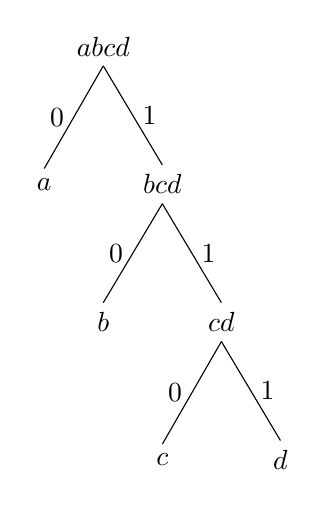
\begin{tikzpicture}[level distance=1.75cm,
	level 1/.style={sibling distance=1.5cm},
	level 2/.style={sibling distance=1.5cm},
	level 3/.style={sibling distance=1.5cm}]
	
	\node (Root) {$abcd$}
	child {
		node {$a$} edge from parent node[left] {0}
	}
	child {
		node {$bcd$}
		child { node {$b$} edge from parent node[left] {0}}
		child { node {$cd$} 
			child {node {$c$} edge from parent node[left] {0} }
			child {node {$d$} edge from parent node[right] {1} }
			edge from parent node[right] {1}}
		edge from parent node[right] {1}
	};
	
	\end{tikzpicture}
	\caption{A Huffman Tree generated for the data `\textbf{aaaabcd}'}
	\label{huff_with_bin}
\end{figure}

In order to generate such a Huffman tree, the frequency of the symbols in the original data must be acquired. For simplistic visualisation, I have displayed the symbols and their frequencies in matrix form as below.
\begin{equation*}
\begin{pmatrix}
a & 4 \\
b & 1 \\
c & 1 \\
d & 1
\end{pmatrix}
\end{equation*}

Now, it is required that we concatenate symbols whilst adding frequencies until we obtain a frequency that matches the original data's length. At each step, the two symbols with the lowest occurrence frequencies should be concatenated \citep{huffman_paper}. \emph{Note: If there is a tie for lowest frequency between 3 or more symbols, any two can be safely chosen}.
\begin{equation}{\label{huff_matrix}}
\begin{pmatrix}
a & 4 \\
b & 1 \\
c & 1 \\
d & 1
\end{pmatrix}
\rightarrow
\begin{pmatrix}
a & 4 \\
b & 1 \\
cd & 2 
\end{pmatrix}
\rightarrow
\begin{pmatrix}
a & 4 \\
bcd & 3
\end{pmatrix}
\rightarrow
\begin{pmatrix}
abcd & 7
\end{pmatrix}
\end{equation}

From these symbol concatenations, working backwards, we are able to generate the associated Huffman tree:

\begin{figure}[H]
	\begin{minipage}{.4\textwidth}
		\begin{equation*}
		\begin{pmatrix}
		abcd
		\end{pmatrix}
		\rightarrow
		\begin{pmatrix}
		a \\
		bcd
		\end{pmatrix}
		\end{equation*}
	\end{minipage}%
	\begin{minipage}{.5\textwidth}
		\begin{figure}[H]
			\centering
			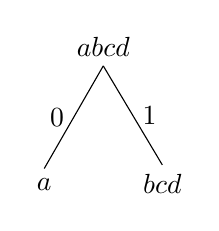
\begin{tikzpicture}[level distance=1.75cm,
			level 1/.style={sibling distance=1.5cm}]
			
			\node (Root) {$abcd$}
			child {
				node {$a$} edge from parent node[left] {0}
			}
			child {
				node {$bcd$} edge from parent node[right] {1}
			};
			
			\end{tikzpicture}
		\end{figure}
	\end{minipage}
\end{figure}
\begin{figure}[H]
	\begin{minipage}{.44\textwidth}
		\begin{equation*}
		\begin{pmatrix}
		a\\
		bcd
		\end{pmatrix}
		\rightarrow
		\begin{pmatrix}
		a\\
		b\\
		cd 
		\end{pmatrix}
		\end{equation*}
	\end{minipage}%
	\begin{minipage}{.5\textwidth}
		\begin{figure}[H]
		\centering
		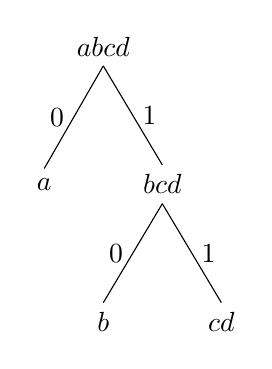
\begin{tikzpicture}[level distance=1.75cm,
		level 1/.style={sibling distance=1.5cm},
		level 2/.style={sibling distance=1.5cm}]
		
		\node (Root) {$abcd$}
		child {
			node {$a$} edge from parent node[left] {0}
		}
		child {
			node {$bcd$} 
			child { node {$b$} edge from parent node[left] {0}}
			child { node {$cd$} edge from parent node[right] {1}}
			edge from parent node[right] {1}
		};
		
		\end{tikzpicture}
		\end{figure}
	\end{minipage}
\end{figure}
\begin{figure}[H]
	\begin{minipage}{.44\textwidth}
		\begin{equation*}
		\begin{pmatrix}
		a\\
		b\\
		cd
		\end{pmatrix}
		\rightarrow
		\begin{pmatrix}
		a\\
		b\\
		c\\
		d
		\end{pmatrix}
		\end{equation*}
	\end{minipage}%
	\begin{minipage}{.5\textwidth}
		\begin{figure}[H]
			\centering
			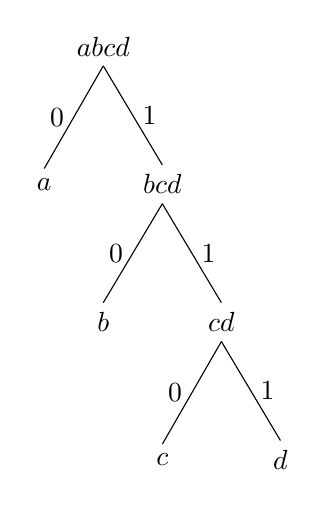
\begin{tikzpicture}[level distance=1.75cm,
			level 1/.style={sibling distance=1.5cm},
			level 2/.style={sibling distance=1.5cm},
			level 3/.style={sibling distance=1.5cm}]
			
			\node (Root) {$abcd$}
			child {
				node {$a$} edge from parent node[left] {0}
			}
			child {
				node {$bcd$}
				child { node {$b$} edge from parent node[left] {0}}
				child { node {$cd$} 
					child {node {$c$} edge from parent node[left] {0} }
					child {node {$d$} edge from parent node[right] {1} }
					edge from parent node[right] {1}}
				edge from parent node[right] {1}
			};
			
			\end{tikzpicture}
		\end{figure}
	\end{minipage}
\caption{Generation of a simple Huffman tree}
\label{simple_huffman}
\end{figure}

A Huffman Tree is traversed from the root node, to each tail node, appending each binary value in order to generate the appropriate code values for the associated symbols \citep[pp.~1100-1101]{huffman_paper}.

Using the bottom tree in Figure \ref{simple_huffman} to generate a code for the symbol `$c$', we obtain the code `$110$' by traversing the tree and concatenating the assigned path bit values. \emph{Note: Switching the paths of the `1's with the paths of the `0's will still result in equally efficient Huffman codes.}

\subsection{Huffman Code Optimality Proof}

Codes generated using the Huffman tree are known to be optimal for any input data and their associated symbol occurrence frequencies. This section provides a written proof of the optimality of binary Huffman codes as referenced from the following book: \citep[p.~41-49]{intro_to_dc} and also from Huffman's original paper itself \citep{huffman_paper}.

Sayood states that the following four conditions are required for an optimal binary Huffman code, each of which can be proven to be satisfied using the Huffman algorithm:

\begin{enumerate}
	\item[\textbf{1.}] Given two letters, denoted by $a_j$ and $a_k$, if the probability $P[a_j]\geq P[a_k]$ then the length of the bit string code representation $l_j \leq l_k$;
\end{enumerate}
If there were such symbols with a higher occurrence than others that had longer code representations than others, the average number of bits per symbol bit string (length) would increase and therefore not be optimal.
\begin{enumerate}
	\item[\textbf{2.}] The two symbols with the lowest frequencies must have the same length $l_m$, where $l_m$ is the maximum possible bit string length for a symbol;
\end{enumerate}
Imagine a situation in which an optimal code $\xi$ exists but the two symbol representations with the lowest frequencies say $a_{m_1}$ and $a_{m_2}$,  do not have the same length. Suppose that $l_{m_2}$ is $k$ number of bits more than that of $l_{m_1}$. Due to the prefix property of Huffman codes, $a_{m_1}$ must not be a prefix of $a_{m_2}$, thus the additional $k$ bits of $a_{m_2}$ can be safely disregarded because the two bit strings would be distinct. As the two symbols associated with $a_{m_1}$ and $a_{m_2}$ occur the least (but at least once) within the source data, the `shortened' bit string would be guaranteed not to be a prefix of any other code. Additionally, disregarding these $k$ bits, a new code can be acquired that has a shorter average length than $\xi$, however this violates our assumption that $\xi$ is an optimal code. This proves that our second condition always holds true for binary Huffman codes.
\begin{enumerate}
	\item[\textbf{3.}] The associated Huffman tree must have two branches (paths) stemming from each intermediate node;
\end{enumerate}
In the case that only one branch (path) extended from an intermediate node, we could remove this path and convert the intermediate node into a leaf node without affecting the decipherability of the code. In turn, this would also reduce the average code length for the given data.
\begin{enumerate}
	\item[\textbf{4.}] Suppose altering an intermediate node into a leaf (or ending) node in the Huffman tree by combining each leaf node protruding from it into a concatenation of symbols (referred to as the reduced alphabet). If the original tree was optimal for the original alphabet, the reduced tree is optimal for the reduced alphabet.
\end{enumerate}
In the event that this condition was not satisfied, a code could be found with a shorter average length for the reduced alphabet. We could then expand the symbol concatenation to obtain a new Huffman tree with a shorter average length than our original `optimum' tree. This would be contradictory to our statement about the optimality of the original tree.

As above, the four conditions stated by Sayood and Huffman can be proven to be satisfied with the Huffman algorithm. Therefore Huffman codes are proven to be optimal for any input data and their associated symbol occurrence frequencies. \hfill$\blacksquare$

\subsection{Efficiency}
Take an example string of data to be encoded, say `\textbf{aabbbccccd}'. The frequencies of each symbol are as follows:
\begin{equation*}
\begin{pmatrix}
a & 2 \\
b & 3 \\
c & 4 \\
d & 1
\end{pmatrix}
\end{equation*}

Concatenating symbols, summing frequencies and generating the Huffman tree:

\begin{minipage}{.5\textwidth}
\begin{equation*}
\begin{pmatrix}
a & 2 \\
b & 3 \\
c & 4 \\
d & 1
\end{pmatrix}
\rightarrow
\begin{pmatrix}
ad & 3 \\
b & 3 \\
c & 4 
\end{pmatrix}
\rightarrow
\begin{pmatrix}
adb & 6 \\
c & 4 
\end{pmatrix}
\rightarrow
\begin{pmatrix}
adbc & 10
\end{pmatrix}
\end{equation*}
\end{minipage}
\begin{minipage}{.5\textwidth}
\begin{figure}[H]
	\centering
	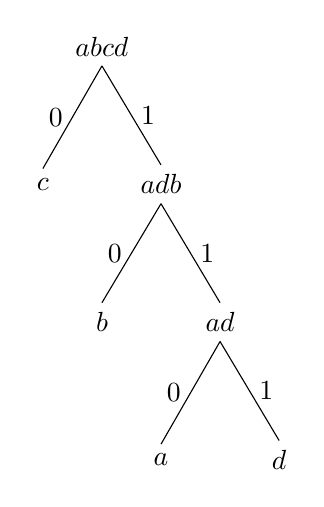
\begin{tikzpicture}[level distance=1.75cm,
	level 1/.style={sibling distance=1.5cm},
	level 2/.style={sibling distance=1.5cm},
	level 3/.style={sibling distance=1.5cm}]
	
	\node (Root) {$abcd$}
	child {
		node {$c$} edge from parent node[left] {0}
	}
	child {
		node {$adb$}
		child { node {$b$} edge from parent node[left] {0}}
		child { node {$ad$} 
			child {node {$a$} edge from parent node[left] {0} }
			child {node {$d$} edge from parent node[right] {1} }
			edge from parent node[right] {1}}
		edge from parent node[right] {1}
	};
	
	\end{tikzpicture}
	\caption{Huffman tree for `\textbf{aabbbccccd}'}
	\label{huff_efficiency}
\end{figure}
\end{minipage}
\hfill\linebreak
Here, the symbol code representations are: 
\begin{table}[H]
	\centering
	\begin{tabular}{|c|c|c|c|c|}
		\hline
		Symbol & a & b & c & d\\
		\hline
		Code & 110 & 10 & 0 & 111\\
		\hline
	\end{tabular}
	\caption{Efficiency example symbols and their assigned codes}
	\label{sym_efficiency}
\end{table}
Therefore the final Huffman encoded data is: `\textbf{1101101010100000111}' (written as a bit string).
The length of the original data is 10 symbols. 

Although symbols are commonly stored using 8 or 16 bits (as in ASCII-8 and UTF-16), we shall assume that the original fixed code length is the minimum possible for the given input data. This is in order to make tests more realistic and fair. The minimum fixed-length value is calculated by taking $\ceil{\log_2{\text{(\#unique\_symbols)}}}$. Let $\ceil{\log_2{\text{(\#unique\_symbols)}}}=M$, then the reason this works is because the number of unique symbols will always be less than or equal to $2^M$, where $2^M$ represents the number of unique binary combinations that can be made \citep{code_definitions}.

For the example, we assume that each code representation in the unencoded data has a fixed-length of $\ceil{\log_2{(4)}}=2$. The unencoded data therefore has a total size of $10\times2 \text{ bits} = 20\text{ bits}$. The encoded data has a length, and therefore size of $19\text{ bits}$, thereby providing a compression rate of $(19\div20)\cdot100 = \textbf{95\%}$. An important remark here, is that the dictionary of symbol-code mappings will need to be stored in addition to the encoded data, thus the rate of compression will be worse (greater) than $95\%$ if applied to this data realistically.

\clearpage
\section{Lempel-Ziv-77 (Sliding Window)}
\subsection{Concept}	
Lempel-Ziv-77 (LZ77) is a lossless, dictionary-based algorithm used for data compression that was initialised by Jacob Ziv and Abraham Lempel in 1977 \citep{lz77}. LZ77 is commonly known as the `sliding window' compression method, due to its unique style of encoding and decoding data - this will be discussed later on in Section \ref{sec_sliding_window}.

The LZ77 algorithm is `dictionary-based' because it uses dictionary coding to encode raw data. Dictionary coding attempts to locate repetitions of a short piece of data within the full dataset, and replaces these repetitions with a reference to a dictionary entry (or token). LZ77 is said to use an `adaptive dictionary' because dictionary entries are created during the encoding process \citep{the_lz_algorithm}. 

\subsection{The `Sliding Window'} \label{sec_sliding_window}

During the encoding and decoding processes of LZ77, there are two important structures, these are \citep[pp.~176]{dc_complete_ref}:

\begin{itemize}
	\item \textbf{Search Buffer}: a string of symbols that have already been read or written by the encoder or decoder. This has a length dependant the implementation and on the specification itself. Larger lengths will typically result in better compression but will take longer to complete encoding;
	
	\item  \textbf{Look-Ahead Window/Buffer}: a string of symbols that have yet to be processed. Once again, the length of the window depends on the implementation and specification. The window length may also be changed depending on requirements for compression or time.
\end{itemize}
Visually, the search buffer and look-ahead window on a piece of data may look as follows (Figure \ref{search_buffer}), where together the search buffer and look ahead window are the two parts of the `sliding window':

\begin{figure}[!h]
	\centering
	\setlength\tabcolsep{1.5pt} % default value: 6pt
	\begin{tabular}{c | c !{\vrule width 1mm} c | c} 
		\cline{2-3}
		& \multicolumn{1}{|c!{\vrule width 1mm}}{Search Buffer} & \multicolumn{1}{ c |}{Look Ahead Window}\\
		\hline
		..abbc & \textbf{aaabbcaaabbbccccaabc} & \textbf{abcaaabbccccaaaabcca} & aabc..\\
		\hline
		\multicolumn{2}{c}{$\leftarrow$ Processed data} & \multicolumn{2}{c}{Data to be processed $\rightarrow$}\\
	\end{tabular}
	\caption{Search Buffer and Look-Ahead Window}
	\label{search_buffer}
\end{figure}

Figure \ref{search_buffer} shows unencoded data being processed with LZ77's sliding window. The entire sliding window `slides' forward one symbol position for each symbol processed and does this until all of the data has been processed \citep[p.~176]{dc_complete_ref}.

\subsection{Token Dictionary} \label{sec_token_dic}

To construct a dictionary of LZ77 tokens, the sliding window should be used. The steps the LZ77 algorithm takes to encode data are \citep[p.~176-177]{dc_complete_ref}:

\begin{enumerate}
	\item Specify a maximum length for the search buffer and look ahead window;
	\item Take a piece of unencoded data consisting of symbols and read the first character - this character is now part of the look ahead window;
	\item If the current symbol is also found in the search buffer, move the sliding window 1 position onwards and perform this check again - go to (3);
	\item If the current symbol is not found in the search buffer, create a token, move the sliding window 1 position onwards - go to (3);
	\item Once all symbols have been processed, stop.
\end{enumerate} 
An example of an LZ77 dictionary creation for the data `\textbf{abcbbabd}' can be seen in Table \ref{dic_code_create} below. \emph{Note: In this example, we set the search buffer and look ahead window to be infinite in length, or at least longer than the original data length.}

\begin{table}[H]
	\centering
	\begin{tabular}{| c | c | c |} 
		\hline
		Step & Unencoded data being processed & $<$Offset, Length, Symbol$>$\\
		\hline
		1 & {\vrule width 0.5mm}\textbf{ a }b c b b a b d & $<$0,0,a$>$\\
		2 & a {\vrule width 0.5mm}\textbf{ b }c b b a b d & $<$0,0,b$>$\\
		3 & a b {\vrule width 0.5mm}\textbf{ c }b b a b d & $<$0,0,c$>$\\
		4 & a \underline{b} c {\vrule width 0.5mm}\textbf{ b }b a b d & $<$-2,1,b$>$\\
		5 & \underline{a b} c b b {\vrule width 0.5mm}\textbf{ a }b d & $<$-5,2,d$>$\\
		\hline
	\end{tabular}
	\caption{LZ77 Dictionary Token Creation}
	\label{dic_code_create}
\end{table}

In Table \ref{dic_code_create}, each bold character represents the next required symbol to be read, whereas each underlined character represents a located symbol match. For the first three steps, there are no matches in the search buffer. 

At step 4, a match for the current symbol is found two characters backwards in the search buffer; this value is known as the offset (offset$=2$). The window then slides forward by one position, providing a new symbol of `b'. However, from the previous match, it's next symbol is `c', therefore the token must be created and the window must be moved on by 1 position - the match length found was 1 character long.

Step 5 presents a similar situation to step 4. The current symbol `a' is matched at offset 5. On sliding one position further the current symbol is now `b', this is the same as the previous match's next character (also `b'). After this, sliding one position provides a current symbol of `d', however the previous match's next character is `c', therefore the token must be created - the match length found was 2. All symbols have been processed thus the algorithm ends. 

In the event that two or more matches are found within the search buffer, the match closest to the look ahead window is chosen. If the chosen match does not contain the next look ahead character, the match one further from the look ahead window is checked.

Now taking the previously created dictionary tokens and using them as a decoding example (Table \ref{dic_code_decode}):

\begin{table}[H]
	\centering
	\begin{tabular}{| c | c | l |} 
		\hline
		Step & $<$Offset, Length, Symbol$>$ & Decoded Data\\
		\hline
		1 & $<$0,0,a$>$ & \textbf{a} \\
		2 & $<$0,0,b$>$ & a\textbf{ b} \\
		3 & $<$0,0,c$>$ & a b\textbf{ c} \\
		4 & $<$-2,1,b$>$ & a \underline{b} c\textbf{ b b}\\
		5 & $<$-5,2,d$>$ & \underline{a b} c b b\textbf{ a b d}\\
		\hline
	\end{tabular}
	\caption{LZ77 Dictionary Token Decoding}
	\label{dic_code_decode}
\end{table}

Step 5 in Table \ref{dic_code_decode} presents us with the correct symbol string. In order to reach this, the following has to be performed: At step 1, the token is read, stating that the offset and length of data match are zero, therefore only the symbol `a' had to be copied. This is also the same for steps 2 and 3 with symbols `b' and `c' respectively.

At step 4, the offset is 2 and the match length is 1, therefore traversing from the end of the string 2 characters, we reach `b'. This `b' is copied, and then the final `b' from the token is copied to the decoded data symbol string.

At step 5, the offset is 5 and the match length is 2. By traversing backwards through the string, we arrive at `a'. The match length is 2, therefore we need to append `a b'. Once this has been appended, the symbol `d' from the token must be copied. All tokens have been read, therefore the decoding is complete.

While this example has provided a specific type of LZ77 encoding, there may be other ways to implement the algorithm. The original paper \citep{lz77} describes a generalisation of the algorithm rather than a specific implementation.

\subsection{Efficiency}

Taking the example data from Section \ref{sec_token_dic} (`\textbf{abcbbabd}') and assuming that each symbol is 1 byte in size. The length of the unencoded data is 8 characters, therefore it has the overall size of $8 \times 8 \text{ bits} =$ \textbf{64 bits}. The token dictionary associated with this data is:

\begin{table}[H]
	\centering
	\begin{tabular}{| c |} 
		\hline
		$<$Offset, Length, Symbol$>$\\
		\hline
		$<$0,0,a$>$\\
		$<$0,0,b$>$\\
		$<$0,0,c$>$\\
		$<$-2,1,b$>$\\
		$<$-5,2,d$>$\\
		\hline
	\end{tabular}
	\caption{LZ77 Example 1 Dictionary}
	\label{dic_ex1}
\end{table}

The dictionary in Table \ref{dic_ex1} contains $3 \times 5 = 15$ symbols. Assuming each symbol is 1 byte in size, the overall size of the encoded data is $15 \times 8 \text{ bits} =$ \textbf{120 bits}.

Of course, this means that the encoded data is $(120\div64)\times100=\textbf{187.5\%}$ of the size of the original data, therefore the data has actually not been compressed. This problem here is that the unencoded data is short and consists of multiple short matches.

For a longer piece of data with longer matches, LZ77 becomes more suitable. Displaying this with another example, say the unencoded data `\textbf{aaaaaaaabbbbbbbaaaaabbbbbbba}'. This data has length 28, therefore assuming a symbol size of 1 byte, the overall data has size $28 \times 8 \text{ bits}=\textbf{224 bits}$. The associated dictionary for this data is:

\begin{table}[H]
	\centering
	\begin{tabular}{| c |} 
		\hline
		$<$Offset, Length, Symbol$>$\\
		\hline
		$<$0,0,a$>$\\
		$<$-1,6,a$>$\\
		$<$0,0,b$>$\\
		$<$-1,5,b$>$\\
		$<$-C,C,a$>$\\
		\hline
	\end{tabular}
	\caption{LZ77 Example 2 Dictionary (Hexadecimal)}
	\label{dic_ex2}
\end{table}

The above dictionary (Table \ref{dic_ex2}) contains $3 \times 5 = 15$ symbols. Assuming each symbol is 1 byte in size, the overall size of the encoded data is $15 \times 8 \text{ bits} =$ \textbf{120 bits}.

In this case, the LZ77 encoded data is $(120\div224)\times100\approx\textbf{53.6\%}$ of the unencoded data's original size. This shows that LZ77 can be efficient, assuming the right type of data.

\clearpage
\section{Lempel-Ziv-4}
\subsection{Concept}	
Lempel-Ziv-4 is a modern compression algorithm based on the ideas presented in LZ77. LZ4 places its focus on the speed of compression and decompression, while still attempting to maintain a good compression ratio \citep{lz4_fpga}. Similarly to LZ77 but unlike Huffman Coding, LZ4 is a dictionary based compression technique.

The official Git-Hub page for LZ4 provides the specification and documentation required to produce a working LZ4 compressor and decompressor. Currently, this compression algorithm is used in a variety of areas including Operating Systems (OS), file systems, games, networking, databases, graphics and caching \citep{lz4_github}.


\subsection{Data Blocks}
LZ4 works using sequences (blocks) of data. Figure \ref{lz4_block} shows the standard LZ4 block format.


\begin{figure}[H]
	\centering
	\begin{tabular}{| c | c | c | c | c |} 
		\hline
		1 byte & 0-$n$ bytes & 0-$L$ bytes & 2 bytes & 0-$n$ bytes\\
		\hline
		Token & Symbol Length+ (optional) & Symbols & Offset & Match Length+ (optional)\\
		\hline
	\end{tabular}
	\caption{LZ4 Standard Data Block Format}
	\label{lz4_block}
\end{figure}

Each item depicted in Figure \ref{lz4_block} is explained in further detail below \citep{how_lz4_works}, \citep{lz4_explained}:

\begin{itemize}
	\item \textbf{Symbols}: The actual character values of the data (for example `$a$', `$2$', `$\pounds$' etc.);
	
	\item \textbf{Token}: a 1 byte field, where the upper 4 bits (of the binary string) describe the frequency of symbols, and the lower 4 bits describe the length of the data/symbol match found\footnote{The match length should not be less than four (as per the specification), therefore a value of `0' in the LZ4 data, represents an actual data match length of `4'. The maximum match length that can be represented in the token alone, is therefore `19' ($15+4$).};
	
	\item \textbf{Symbol Length+}: Extra allocated block space in the event that the frequency of symbols exceeds the maximum of 15 (1111) allocated in the token;
	
	\item \textbf{Offset}: The number of data positions to traverse in the current decoded data from the tail end, towards the beginning (little endian); 
	
	\item \textbf{Match Length+}: Extra allocated space in the event that the length of the data match exceeds the maximum of 15 (1111) allocated in the token.
\end{itemize}

One restriction of the format of the data (as per the specification) is that the final five bytes of data (at least), must be uncompressed \citep{lz4_github}.
If there is to be more than one data block in the LZ4 data, these blocks are concatenated in series, one after the other. In order to identify where the LZ4 data ends, a specific ``Ending Marker" has to be used. This ``Ending Marker" is specified to be four null (zero) bytes (`\textbf{00 00 00 00}').


\subsection{Compression Example}{\label{sec_lz4_compress}}
This example will take a piece of uncompressed data and apply LZ4 compression to it. See Figure \ref{uncompressed_lz4} below for data position references and the uncompressed data.

\begin{figure}[H]
	\centering
	\setlength\tabcolsep{3pt} % default value: 6pt
	\begin{tabular}{|c|c|c|c|c|c|c|c|c|c|c|c|c|c|c|c|c|c|c|c|} 
		\hline
		\textbf{Position} & 1 & 2 & 3 & 4 & 5 & 6 & 7 & 8 & 9 & 10 & 11 & 12 & 13 & 14 & 15 & 16 & 17 & 18 & 19\\
		\hline
		\textbf{Data} & a & b & b & c & c & a & b & b & c & c & c & a & b & b & a & a & b & c & c\\
		\hline
	\end{tabular}
	\caption{Uncompressed data to be encoded with LZ4}
	\label{uncompressed_lz4}
\end{figure}

\begin{itemize}
	\item Reading the data per symbol, the first match ($\geq$ length 4) is located when reaching position 6 in the data - `\textbf{abbcc}' have been read. The match is found at position 1 (offset 5);
	\item Similarly to the LZ77 process, the position is incremented by 1 and a symbol match is searched for in the previous data. In this case, the full match is from position 6-10 (matches with position 1-5);
	\item Creating the data block:
		\begin{itemize}
			\item The symbols are: \textbf{abbcc};
			\item The length of symbols is \textbf{5} (hexadecimal);
			\item The match length is 5 - therefore the low token value will be $5-4=\textbf{1}$ (hexadecimal);
			\item The offset is \textbf{05 00} (hexadecimal - little endian).
		\end{itemize}
	\item Overall, the first data block is `\textbf{51 abbcc 05 00}'.
	\item Progressing to position 11 - `\textbf{abbccabbcc}' have been read. The closest match ($\geq$ length 4) is located at position 5 (offset 6);
	\item Incrementing the position and searching for symbol matches, it is found that position 11-14 matches with position 5-8;
	\item Creating the data block:
		\begin{itemize}
			\item No symbols were found before a match was located after creating the previous data block;
			\item The length of symbols is \textbf{0} (hexadecimal);
			\item The match length is 4 - therefore the low token value will be $4-4=\textbf{0}$ (hexadecimal);
			\item The offset is \textbf{06 00} (hexadecimal - little endian).
		\end{itemize}
	\item Overall, the second data block is `\textbf{00 06 00}' (no symbols);
	\item The remaining data is located within the final five bytes of data, therefore it should be left uncompressed as `\textbf{aabcc}'.
	\item Concatenating the data blocks and appending the ``Ending Marker", the final LZ4 data is: `\textbf{51 abbcc 05 00 00 06 00 aabcc 00 00 00 00}'.
\end{itemize}

\subsection{Decompression Example}
This example will decompress the data from Section \ref{sec_lz4_compress}. For clarity, the LZ4 data is located in Figure \ref{lz4_encoded} below:

\begin{figure}[H]
	\centering
	\setlength{\tabcolsep}{2.5pt}
	\begin{tabular}{|c | c | c | c | c | c | c  c  c|}
		\hline
		\text{Token}&
		\text{Symbols}&
		\text{Offset}&
		\text{Token}&
		\text{Offset}&
		\text{Symbols}&
		\multicolumn{3}{c|}{Ending Marker}
		\\
		\hline
		\textbf{51} & 
		\textbf{abbcc} & 
		\textbf{05 00} & 
		\textbf{00} & 
		\textbf{06 00} &
		\textbf{aabcc}&
		\multicolumn{3}{c|}{\textbf{00 00 00 00}}\\
		\hline
	\end{tabular}
	\caption{LZ4 encoded data to be decompressed}
	\label{lz4_encoded}
\end{figure}

\emph{Note: Each numeric value in Figure \ref{lz4_encoded} is written in hexadecimal.}
\\\\
Decoding the data:
\begin{itemize}
	\item Reading the first data block `\textbf{51 abbcc 05 00}'. The following information can be extracted:
		\begin{itemize}
			\item The length of symbols to copy is \textbf{5};
			\item The symbols are `\textbf{abbcc}';
			\item The length of the symbol match is $1+4=\textbf{5}$;
			\item The symbol match begins at offset \textbf{5};
		\end{itemize}
	\item Applying this information, the following decompressed data is generated - `\textbf{abbccabbcc}';
	\item Reading the second data block `\textbf{00 06 00}'. The following information can be extracted:
		\begin{itemize}
			\item The length of symbols to copy is \textbf{0};
			\item The are no symbols to copy;
			\item The length of the symbol match is $0+4=\textbf{4}$;
			\item The symbol match begins at offset \textbf{6};
		\end{itemize}
	\item Applying this information to the previously uncompressed data, the uncompressed data is now - `abbccabbcc\textbf{cabb}';
	\item The next block is fully uncompressed, therefore this should be appended to the current decompressed data - `abbccabbcccabb\textbf{aabcc}';
	\item The next block is the ending marker, therefore all of the LZ4 data has been successfully decompressed. The final decompressed data is: `\textbf{abbccabbcccabbaabcc}'.
\end{itemize}

\subsection{Efficiency}
Working with the example uncompressed data `\textbf{abbccabbcccabbaabcc}', this has a length of 19 symbols. Once again assuming that each symbol consists of 1 byte (8 bits each), the overall size of the data is $19\times8\text{ bits}=\textbf{152 bits}$.

The LZ4 encoded data `\textbf{51 abbcc 05 00 00 06 00 aabcc 00 00 00 00}' has a byte length (assuming each symbol is a byte) of 20. Translating this into bits, the LZ4 encoded data has a size of $20\times8\text{ bits}=\textbf{160 bits}$.

Overall efficiency the LZ4 encoded data is $(160\div152)\times100\approx\textbf{105\%}$ of the size of the uncompressed data. This means that the data has not been compressed, however in the event that the uncompressed data is longer and matches are also longer, LZ4 can provide a reasonable compression very efficiently due to it being based on LZ77.


\clearpage
\section{Implementations}
\subsection{Huffman Encoder}{\label{sec_huff_enc}}

This section explains my Huffman Encoder implementation running on a test file. Each implementation is written using the Octave programming language, however only generalisations are given, therefore any programming language can be used. My implementation takes any input file, such as `poem.txt' and reads the raw data of this file in as an array of bytes. It is intentional that the raw data of the file is read, so that any file format is supported. An example of this raw data array is as follows, where each numeric value is a decimal representation of the actual symbols in the source file:

\begin{minted}[frame=single, breaklines]{octave}
input_data = [67 111 109 112 32 115 ...]'
\end{minted}

Once the input\_data array has been populated, a new array is created, containing only unique symbol values from the input array in raw byte value ascending order.

\begin{minted}[frame=single, breaklines]{octave}
symbols = [10 13 32 33 34 39 44 45 ...]'
\end{minted}

 The next array to be produced is one containing references to the `symbols' array row entries (column 1), with their frequencies of occurrence (column 2) from the source data. This array is sorted in ascending order of frequency. A copy is made of the array for future reference.

\begin{minted}[frame=single, breaklines]{octave}
unique_data_sorted =
 ...
 12     4 %e.g. symbol at row 12 in 'symbols' occurs 4 times
 17     4 %...  
 11     5 %...  symbol at row 11 in 'symbols' occurs 5 times
 21     5 %...
 5      6 %...  symbol at row 5 in 'symbols' occurs 6 times
 8      7 %...
 ...
\end{minted}

Now a new array is created, `tree\_struct'. This array defines the structure of the Huffman Tree. Concatenating symbols from the unique sorted array based on smallest frequencies in the array (as in Section \ref{sec_huff_trees}, equation (\ref{huff_matrix})), `tree\_struct' is populated. At each stage, the two concatenated symbols are changed to the value of a reference counter (which starts at -1 and decreases by 1 when a concatenation occurs) and the original symbol row entries are deleted from the array.

\begin{figure}[H]
\begin{minipage}{0.5\textwidth}
\centering
[symbol, frequency]
\begin{minted}[frame=single, breaklines]{octave}
	unique_data_sorted =
	4      1
	13     1
	16     1
	20     1
	...
	\end{minted}
\end{minipage}
\begin{minipage}{0.5\textwidth}
\centering
[symbol 1, symbol 2]
\begin{minted}[frame=single, breaklines]{octave}
	tree_struct = []
	
	
	
	
	
\end{minted}
\end{minipage}
\begin{minipage}{0.5\textwidth}
	\centering
	\begin{minted}[frame=single, breaklines]{octave}
	unique_data_sorted =
	16     1
	20     1
	23     1
	47     1
	...
	\end{minted}
\end{minipage}
\begin{minipage}{0.5\textwidth}
	\centering
	\begin{minted}[frame=single, breaklines]{octave}
	tree_struct = 
	4     13 %two lowest freqs.
	
	
	
	
	\end{minted}
\end{minipage}
\begin{minipage}{0.5\textwidth}
	\centering
	\begin{minted}[frame=single, breaklines]{octave}
	unique_data_sorted =
	23     1
	47     1
	49     1
	-2     2 %concat'd symb. ref
	...
	\end{minted}
\end{minipage}
\begin{minipage}{0.5\textwidth}
	\centering
	\begin{minted}[frame=single, breaklines]{octave}
	tree_struct = 
	4     13	
	16    20 %two lowest freqs.
	
	
	
	\end{minted}
\end{minipage}
\begin{minipage}{0.5\textwidth}
	\centering
	\begin{minted}[frame=single, breaklines]{octave}
	unique_data_sorted =
	49     1
	-3     2 %concat'd symb. ref
	-2     2 %...
	-1     2 %...
	...
	\end{minted}
\end{minipage}
\begin{minipage}{0.5\textwidth}
	\centering
	\begin{minted}[frame=single, breaklines]{octave}
	tree_struct = 
	4     13	
	16    20
	23    47 %two lowest freqs.
	
	
	\end{minted}
\end{minipage}
\begin{minipage}{0.5\textwidth}
	\centering
	\begin{minted}[frame=single, breaklines]{octave}
	unique_data_sorted =
	-2     2 %concat'd symb. ref
	-1     2 %...
	18     2
	-4     3 %...
	...
	\end{minted}
	...
\end{minipage}
\begin{minipage}{0.5\textwidth}
	\centering
	\begin{minted}[frame=single, breaklines]{octave}
	tree_struct = 
	4     13	
	16    20
	23    47 
	49    -3 %two lowest freqs.
	
	\end{minted}
	...
\end{minipage}
\caption{Generating the Huffman Tree structure as an array}
\end{figure}

Now that the Huffman Tree structure has been generated, the structure must be somehow `traversed' in order to generate the Huffman codes for each unique symbol in the original data. This process, using pseudo-code is as follows (Figure \ref{huff_codes_psuedo}):

\begin{figure}[H]
\begin{minted}[frame=single, breaklines, linenos]{octave}
%initialise cell arrays
codes; prefixes;

for each row in unique_data_sorted:

 if the value in column 1 is positive:
  column 1 symbol code = its previous code value append '1'
 else
  column 1 symbol prefix = (its previous code value append its previous code value) append '1'
 end
 
 if the value in column 2 is positive:
  column 2 symbol code = its previous code value append '0'
 else
  column 2 symbol prefix = (its previous code value append its previous code value) append '0'
 end
 
end
\end{minted}
\caption{Pseudo-code for Huffman Tree structure traversal}
\label{huff_codes_psuedo}
\end{figure}

Visualising `tree\_struct' as a Huffman Tree, from the root (end of the array):

\begin{figure}[H]
\begin{minipage}{0.5\textwidth}
	\centering
	\begin{minted}[frame=single, breaklines]{octave}
	tree_struct = 
	...
	-41    3
	-42  -43
	-44  -45
	-46  -47
	\end{minted}
\end{minipage}
\begin{minipage}{0.5\textwidth}
	\begin{figure}[H]
		\centering
		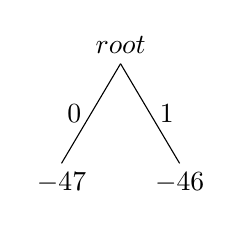
\begin{tikzpicture}[level distance=1.75cm,
		level 1/.style={sibling distance=1.5cm}]
		
		\node (Root) {$root$}
		child {
			node {$-47$} edge from parent node[left] {0}
		}
		child {
			node {$-46$} edge from parent node[right] {1}
		};
		\end{tikzpicture}
	\end{figure}
\end{minipage}
\end{figure}

\begin{figure}[H]
\begin{minipage}{0.5\textwidth}
	\centering
	\begin{minted}[frame=single, breaklines]{octave}
	tree_struct = 
	...
	-39  -40
	-41    3
	-42  -43
	-44  -45
	...
	
	\end{minted}
\end{minipage}
\begin{minipage}{0.5\textwidth}
	\begin{figure}[H]
	\centering
	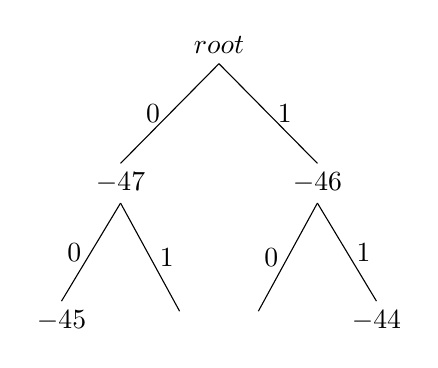
\begin{tikzpicture}[level distance=1.75cm,
		level 1/.style={sibling distance=2.5cm},
		level 2/.style={sibling distance=1.5cm}]
		
		\node (Root) {$root$}
		child {
			node {$-47$} 
			child { node {$-45$} edge from parent node[left] {0}}
			child { node {} edge from parent node[right] {1}}
			edge from parent node[left] {0}
		}
		child {
			node {$-46$} 
			child { node {} edge from parent node[left] {0}}
			child { node {$-44$} edge from parent node[right] {1}}
			edge from parent node[right] {1}
		};
		
	\end{tikzpicture}
	\end{figure}
\end{minipage}
\end{figure}

\begin{figure}[H]
\begin{minipage}{0.5\textwidth}
	\centering
	...
	\begin{minted}[frame=single, breaklines]{octave}
	tree_struct =
	4   13
	...
	
	
	
	
	\end{minted}
\end{minipage}
\begin{minipage}{0.5\textwidth}
	\centering
	...
	\begin{figure}[H]
		\centering
		\begin{tikzpicture}[level distance=1.75cm,
		level 1/.style={sibling distance=4.5cm},
		level 2/.style={sibling distance=1.5cm}]
		
		% The root is made invisible 
		\node {}
		child {node {...} 
			child {node {13} edge from parent node[left] {0}} 
			child {node {...} edge from parent node[right] {1}} 
			edge from parent[draw=none] 
		} 
		child {node {...} 
			child {node {...} edge from parent node[left] {0}} 
			child {node {4} edge from parent node[right] {1}} 
			edge from parent[draw=none] 
		}; 
		
		\end{tikzpicture}
	\end{figure}
\end{minipage}
\caption{Huffman Tree from tree\_struct}
\label{huff_tree_imp}
\end{figure}

Figure \ref{huff_tree_imp} above, shows that the symbol values corresponding to `13' and `4' would be the final leaf nodes appended to the tree visualisation if it were created by hand. This is due to their frequency of occurrence being the lowest of all existing symbols in the source data. Until a positive value is reached in `tree\_struct', no codes are created, only prefixes (that are incidentally stored in the `prefixes' array). 

Based on the tree structure and the pseudo-code presented in Figure \ref{huff_codes_psuedo}, the `codes' array develops into the following, where the code from each row matches respectively with the symbol from the same row in the `symbols' array.

\begin{figure}[H]
\begin{minipage}{0.5\textwidth}
	\begin{minted}[frame=single, breaklines]{octave}
	codes =
	{
	[1,1] = 010010
	[1,2] = 010001
	[1,3] = 000
	[1,4] = 001100000101
	[1,5] = 001100101
	[1,6] = 10001111
	[1,7] = 0010101
	[1,8] = 001100100
	[1,9] = 100110
	[1,10] = 0011001101
	...
	\end{minted}
\end{minipage}
\begin{minipage}{0.5\textwidth}
	\begin{minted}[frame=single, breaklines]{octave}
	symbols =
	
	10
	13
	32
	33
	34
	39
	44
	45
	46
	58
	...
	\end{minted}
\end{minipage}
\end{figure}

The data above is stored in a separate dictionary file to the encoded data itself. This is practically inconvenient, however it is useful for debugging my code. The encoded data is stored in another file with the form as below.

\begin{figure}[H]
\begin{minted}[frame=single]{text}
001100000010100011111000100001100010000110100001110010001100000110001000011
010011001001001111101000001100100001100100001100100000011100000100101000100
110011100100110011010100000111100000001000101010111001111010001010010010001
010010001100000010100011111000100011100101111011010001100010000110111100100
010000111000110111000000111001010000101000110111101001...
\end{minted}
\end{figure}

\subsection{Huffman Decoder}{\label{sec_huff_decoder}}

This section explains the provided the code I have used to produce a working Huffman decoder. My decoder takes two input files, these being the `encoded\_data' and the `dictionary' files, and uses them together to produce the decompressed data. These files contain the encoded Huffman data and associated dictionary respectively.

I shall be following this example using the test file `poem.txt'. To decode the data, I import the `dictionary' as a cell array and the `encoded\_data' as a string. \emph{Remark: I chose a cell array for the dictionary in order to maintain any leading zeroes; a regular array does not cater for this in Octave.}

\begin{figure}[H]
	\begin{minted}[frame=single, breaklines]{octave}
	symbol_dictionary =
	{			         ...
	[1,1] = 10			[1,2] = 010010
	[2,1] = 13			[2,2] = 010001
	[3,1] = 32			[3,2] = 000
	[4,1] = 33			[4,2] = 001100000101
	[5,1] = 34			[5,2] = 001100101
	[6,1] = 39			[6,2] = 10001111
	[7,1] = 44			[7,2] = 0010101
	[8,1] = 45			[8,2] = 001100100
	[9,1] = 46			[9,2] = 100110
	[10,1] = 58       		[10,2] = 0011001101
	...			       ...
	\end{minted}
\end{figure}

\begin{figure}[H]
\begin{minted}[frame=single, breaklines]{octave}
%encoded_data
001100000010100011111000100001100010000110100001110010001100000110001000011
010011001001001111101000001100100001100100001100100000011100000100101000100
110011100100110011010100000111100000001000101010111001111010001010010010001
010010001100000010100011111000100011100101111011010001100010000110111100100
010000111000110111000000111001010000101000110111101001...
\end{minted}
\end{figure}

My next step is to sort the dictionary array based on the length of the binary representations (ascending). I used a bubble sort for this process for simplicity. The reason the data is sorted as such, is to reduce decoding operation time. Symbols that occur most frequently have the shortest binary length; having these symbols at the beginning of the array will mean that when searching for a match, fewer rows will have to be checked for a symbol match.

\begin{figure}[H]
	\begin{minted}[frame=single, breaklines]{octave}
	symbol_dictionary = %sorted
	{				  ...
	[1,1] = 32			 [1,2] = 000
	[2,1] = 101			[2,2] = 111
	[3,1] = 97			 [3,2] = 0111
	[4,1] = 104			[4,2] = 1011
	[5,1] = 105			[5,2] = 1101
	[6,1] = 111			[6,2] = 1010
	[7,1] = 115			[7,2] = 1100
	[8,1] = 116			[8,2] = 0101
	[9,1] = 100			[9,2] = 01100
	[10,1] = 114		       [10,1] = 01101
	...				...
	\end{minted} 
\end{figure}

The penultimate step is to read the encoded data string sequentially per binary character. After reading each character, if there is a match found within the symbol\_dictionary array, append the associated symbol to an output array `decoded\_data'. The psuedo-code (Figure \ref{huff_codes2syms_psuedo}) and an example of this process is explained below.

\begin{figure}[H]
\begin{minted}[frame=single, breaklines, linenos]{octave}
%reading each character from the encoded_data array

for each character:

 if the current character or a concatenation of previous characters fully matches with ONLY ONE Huffman code from the dictionary:
 
 	append the associated symbol to the decoded_data array
  
 else
 
 	move position to the next character
  
 end
end	
\end{minted}
\caption{Pseudo-code to match encoded data with Huffman codes}
\label{huff_codes2syms_psuedo}
\end{figure}

I will use the above process from above (Figure \ref{huff_codes2syms_psuedo}) to find an associated symbol from the sample data.

\begin{figure}[H]
\begin{minted}[frame=single]{text}
...1010001111100010000110... %encoded_data sample
\end{minted}
\begin{minted}[frame=single, breaklines]{octave}
symbol_dictionary =
{				  ...
[1,1] = 32			 [1,2] = 000
[2,1] = 101			[2,2] = 111
[3,1] = 97			 [3,2] = 0111
[4,1] = 104			[4,2] = 1011
[5,1] = 105			[5,2] = 1101
[6,1] = 111			[6,2] = 1010
[7,1] = 115			[7,2] = 1100
[8,1] = 116			[8,2] = 0101
...				...
\end{minted} 
\end{figure}

Reading the first character in the data sample, this matches with the first character of five of the displayed Huffman codes.

\begin{figure}[H]
\begin{minted}[frame=single, escapeinside=||]{text}
...|\bf{1}|010001111100010000110... %encoded_data sample
\end{minted}
\begin{minted}[frame=single, breaklines, escapeinside=||]{octave}
symbol_dictionary =
{				  ...
[1,1] = 32			 [1,2] = 000
[2,1] = 101			[2,2] = |\bf{1}|11  %matched
[3,1] = 97			 [3,2] = 0111
[4,1] = 104			[4,2] = |\bf{1}|011 %matched
[5,1] = 105			[5,2] = |\bf{1}|101 %matched
[6,1] = 111			[6,2] = |\bf{1}|010 %matched
[7,1] = 115			[7,2] = |\bf{1}|100 %matched
[8,1] = 116			[8,2] = 0101
...				...
\end{minted} 
\end{figure}

Continuing the process, the character match `10' now only matches with two of the displayed Huffman codes.

\begin{figure}[H]
\begin{minted}[frame=single, escapeinside=||]{text}
...|\bf{10}|10001111100010000110... %encoded_data sample
\end{minted}
\begin{minted}[frame=single, breaklines, escapeinside=||]{octave}
symbol_dictionary =
{				  ...
[1,1] = 32			 [1,2] = 000
[2,1] = 101			[2,2] = 111
[3,1] = 97			 [3,2] = 0111
[4,1] = 104			[4,2] = |\bf{10}|11 %matched
[5,1] = 105			[5,2] = 1101
[6,1] = 111			[6,2] = |\bf{10}|10 %matched
[7,1] = 115			[7,2] = 1100
[8,1] = 116			[8,2] = 0101
...				...
\end{minted} 
\end{figure}

The next step is to check the next character in the encoded data string.

\begin{figure}[H]
\begin{minted}[frame=single, escapeinside=||]{text}
...|\bf{101}|0001111100010000110... %encoded_data sample
\end{minted}
\begin{minted}[frame=single, breaklines, escapeinside=||]{octave}
symbol_dictionary =
{				  ...
[1,1] = 32			 [1,2] = 000
[2,1] = 101			[2,2] = 111
[3,1] = 97			 [3,2] = 0111
[4,1] = 104			[4,2] = |\bf{101}|1 %matched
[5,1] = 105			[5,2] = 1101
[6,1] = 111			[6,2] = |\bf{101}|0 %matched
[7,1] = 115			[7,2] = 1100
[8,1] = 116			[8,2] = 0101
...				...
\end{minted} 
\end{figure}

This final step finds a symbol match for the encoded concatenation of characters `1010'.

\begin{figure}[H]
\begin{minted}[frame=single, escapeinside=||]{text}
...|\bf{1010}|001111100010000110... %encoded_data sample
\end{minted}
\begin{minted}[frame=single, breaklines, escapeinside=||]{octave}
symbol_dictionary =
{				  ...
[1,1] = 32			 [1,2] = 000
[2,1] = 101			[2,2] = 111
[3,1] = 97			 [3,2] = 0111
[4,1] = 104			[4,2] = 1011
[5,1] = 105			[5,2] = 1101
[6,1] = |\bf{111}|			[6,2] = |\bf{1010}| %matched
[7,1] = 115			[7,2] = 1100
[8,1] = 116			[8,2] = 0101
...				...
\end{minted} 
\end{figure}

Concluding, from the sample piece of data, the first symbol to be found is the symbol corresponding to the decimal value `111'. In the ASCII-8 convention, this is the symbol `o'.

Once the entire encoded\_data array has been traversed, the final step is to save the decoded\_data array in a new file. This is appropriately saved to a new directory with the name `poem\_decoded.txt'. This file is identical to the original `poem.txt' due to Huffman Coding being a lossless compression algorithm.

\subsection{LZ4 Encoder}{\label{sec_lz4_encoder}}

As with my Huffman Encoder implementation (Section \ref{sec_huff_enc}), my LZ4 encoder begins by reading an input file as raw data (a series of bytes). This raw data is stored in an array, `data'. A key part of any LZ4 encoder, is finding sequences of symbol matches within the data. This implementation makes use of a cell array, `matches' for storing the offset and length of matches found at particular positions in the data. Using the data `\textbf{aabbccaabbcabbca}', my `data' and `matches' arrays are as seen below. \emph{Note: the data has been imported as raw data, and is shown as an array of bytes.}

\begin{figure}[H]
\begin{minted}[frame=single]{text}
data = [97 97 98 98 99 99 97 97 98 98 99 97 98 98 99 97]'
\end{minted}
\begin{minted}[frame=single, breaklines]{octave}
matches =
{
[1,1] = [](0x0) %at pos. 1 there are no previous matches >= 4 in length
[1,2] = [](0x0) %at pos. 2 there are no previous matches >= 4 in length
[1,3] = [](0x0) % ...
[1,4] = [](0x0)
[1,5] = [](0x0)
[1,6] = [](0x0)
[1,7] =
	[-6   5] %at pos. 7, there is a match at offset 6 with length 5
[1,8] =
	[-6   4] %at pos. 8, there is a match at offset 6 with length 4
...
[1,12] =
	[-4    5  -10    4] %format [offset match_len; offset match_len] used when more than one match is found
...
\end{minted}
\end{figure}

As to be partially compliant with the LZ4 specification \citep{lz4_github}, and to be compliant with my decoder, I have decided to implement the initial `LZ4 validation check'. This requires the first four bytes within the file to be (little endian, hexadecimal format): `0x184D2204'. The encoder creates a new array, `encoded\_data' and pastes the following at the beginning.

\begin{minted}[frame=single]{text}
encoded_data = [04 22 4D 18 00 00 00 00 00 00 00]
\end{minted}

Note that the trailing `00' byte values are where other parts of the specification are addressed, however these parameters are out of scope for this project and therefore can be ignored.

The next task for the encoder is to traverse the `matches' array and choose the match at each position in the data, where the match length is largest in value. For example, at position 7, the match length `5' and its associated offset `-6' is chosen.

\begin{minted}[frame=single, breaklines, escapeinside=||]{octave}
[1,7] =
	[-6    5]
\end{minted}

Using the match specified, the `data' array can be utilised once again to obtain the symbols. From the match above, the symbols [97 97 98 98 99] are found as the match when searching from position 7 to position 12 in the data.

\begin{minted}[frame=single, escapeinside=||]{octave}
data = [|\emph{\underline{97 97 98 98 99} 99}| |\bf{\underline{97}}||\underline{ }||\underline{97 98 98 99}| 97 98 98 99 97]'
\end{minted}

Now, the encoder has all of the information required to generate an LZ4 data block. Again, for the position 7 example, the block components are:

\begin{minted}[frame=single, escapeinside=||]{octave}
high token value = 6 %length of symbols, hexadecimal value
low token value = 1 %match length - 4, hexadecimal value
symbols to copy = [97 97 98 98 99 99]
offset = 06 00 %little endian, hexadecimal
\end{minted}

Overall, the data block is:

\begin{minted}[frame=single, escapeinside=||]{octave}
[61 97 97 98 98 99 99 06 00]
\end{minted}

This block is appended to the end of the `encoded\_data' array. After working with the current data, the `match' array position is increased to the current position, plus the length of the data match found.

Once complete, the encoded\_data has four null bytes appended to it [00 00 00 00]. Again, this is to partially satisfy the specification and my decoder implementation. Overall, the encoded data will look as follows. 

\begin{minted}[frame=single, breaklines]{text}
[04 22 4D 18 00 00 00 00 00 00 00 61 61 61 62 62 63 63 06 00 01 04 00 00 00 
 00 00]
 %all symbol values are converted to hexadecimal on writing the file
\end{minted}

\subsection{LZ4 Decoder}{\label{sec_lz4_decoder}}

This section explains my implementation of an LZ4 decoder, implemented based on the LZ4 specification found on GitHub \citep{lz4_github}.

The first step taken in the decoding process (after reading the `.lz4' file in as an array of bytes) is to open the specified file and verify that the contents mark it as valid LZ4 data. A valid LZ4 file will always begin with the sequence of bytes [04 22 4D 18] in hexadecimal. If the first four bytes are not these values, it is not a valid LZ4 file. For my implementation of LZ4, we can safely ignore any flags given before the compressed data blocks begin (between bytes 5 and 11 inclusive). \emph{Remark: When reading a file in as raw data, Octave converts hexadecimal values into decimal.}

The decoder now works through each block individually. Let us take the following block from `poem\_encoded.lz4' as an example.

\begin{minted}[frame=single, breaklines]{text}
[... 73 4E 65 74 77 6F 72 6B 5C 00 ...] %all values in hexadecimal
\end{minted}

Before working through this data block, it is necessary to be aware that the decoded data is stored in a cell array, `decoded\_array'.

Reading the first byte `73', the high\_token is set to `\textbf{7}' and the low\_token is set to `\textbf{3}'. The data position is then incremented. As the high\_token does not have the value 'F' (decimal 15), we know that the next byte is the first symbol. The symbols within the data are (reading high\_token = 7 bytes):

\begin{minted}[frame=single, breaklines]{text}
[4E 65 74 77 6F 72 6B] %all values in hexadecimal
\end{minted}

Copying these values to the decoded\_array as symbols (the Octave function `char' uses ASCII-8\footnote{``https://octave.org/doc/v4.0.0/Concatenating-Strings.html"}):

\begin{minted}[frame=single, breaklines]{text}
decoded_array = [... N e t w o r k]' %all values converted to symbols 
\end{minted}

Now the data position moves to one byte after the final symbol representation. To calculate the offset (written as 2-bytes in little endian), both the current and next bytes should be converted to decimal and summed correctly. In this case, the offset bytes are:

\begin{minted}[frame=single, breaklines]{text}
[5C 00] %in hexadecimal, corresponds to decimal offset = 92+(256*0)=92
\end{minted}

Traversing backwards 92 positions in the current decoded\_array, we find the low\_token + 4 ($3+4=7$) symbol values to copy - these are underlined. \emph{Note: If low\_token were to be equal to 15, the byte following the offset would have to be converted to decimal and added to the current low\_token value.}

\begin{minted}[frame=single, breaklines, escapeinside=||]{text}
decoded_array = [... s c i |\underline{\textvisiblespace i s \textvisiblespace s o \textvisiblespace}| h a ...]'
\end{minted}

Appending the located symbols to the end of the decoded\_array:

\begin{minted}[frame=single, breaklines, escapeinside=||]{text}
decoded_array = [... N e t w o r k |\textvisiblespace| i s |\textvisiblespace| s o |\textvisiblespace| ]' %all values as symbols 
\end{minted}

This data block has now been successfully decoded, this process now repeats on trailing data blocks until the offset is found to be equal to zero. This condition indicates the ending marker of the data.

\clearpage
\section{Compression Analysis}

I have chosen a number of test files of uncompressed formats for testing my compressors (Appendix A). I made an informed decision to select a variety of different formats of files with varying content. Some of the test files selected originate from the Canterbury Corpus website \citep{canterbury_corpus}. This website provides corpora used for testing various data compressor implementations. I have made sure to select files of 64KB (kilobytes) or less in size as to satisfy my implementation of the LZ4 specification.
\subsection{Huffman Encoder}
\subsubsection{8-Bit Fixed-Length Code Comparison}
The following pseudo-code describes how the compression levels for my Huffman encoder are calculated against the original data when an 8-bit fixed-length size is assumed for each symbol (for example as in an ASCII-8 system).
\\\textbf{Compression Evaluation Pseudo-Code [8-bit Fixed Length Codes]:}
\begin{minted}[frame=single, breaklines]{octave}
Obtain the file size of the original file;
Obtain the file size of the compressed binary data file;
Obtain the file size of the dictionary file;

%This gives the compression as a percentage of the original file size
Compression = [(compressed_size + dictionary_size)/ original_file_size]*100

\end{minted}

I have evaluated the compression on a variety of test files. The details of these test files are located in Appendix A. Table \ref{huff_enc_results} displays the results of my Huffman encoder on the test files, where the original file size is assumed to consist of symbols with 8-bit code representations (for example as in ASCII-8). 

The table shows us that each test file has been successfully compressed (to less than 100\% of its original size). The file that has been compressed most is `a0270.txt' (14.72\%). This is intuitive as `a0270.txt' consists of 270 counts of only one symbol (`$a$'); therefore each of these symbols can be represented with a 1 bit code, rather than the original 8 bits. Another interesting file here is `ico.bmp'. Although the original file size is large in comparison to `a0270.txt', its compression rate is comparable (23.41\%). Due to how the Huffman algorithm generates variable-length codes for each symbol, it is clear that the symbol alphabet of `ico.bmp' is smaller in size when compared to some of the other test files with a higher compression rate and similar initial file size (such as `fields.c').

Table \ref{huff_enc_results} also shows that for my implementation and the test files, the larger the file size, the longer the runtime. I have decided to use the median value for the averages in this case, as the mean average could be skewed by a considerable amount due to extreme cases.

\begin{table}[H]
	\centering
	\begin{tabular}{| c | c | c | c | c |} 
		\hline
		File-Name & 8-bit Fixed-Length & Encoded Size & Run-Time(s) & Compression\\
		& Size (bits) & (bits) & & \\
		\hline
		a0020.txt & 160 & 68 & 0.02 & 42.50\%\\
		\hline
		a0270.txt & 2160 & 318 & 0.16 & 14.72\%\\
		\hline
		cp.html & 196824 & 139004 & 28.90 & 70.62\%\\
		\hline
		fields.c & 89200 & 66014 & 13.08 & 74.01\%\\
		\hline
		grammar.lsp & 29768 & 25772 & 4.37 & 86.58\%\\
		\hline
		ico.bmp & 103344 & 24195 & 14.44 & 23.41\%\\
		\hline
		obj1 & 172032 & 159288 & 25.30 & 92.59\%\\
		\hline
		paper1 & 425288 & 277404 & 61.50 & 65.23\%\\
		\hline
		poem.txt & 20624 & 16656 & 3.01 & 80.76\%\\
		\hline
		progc & 316888 & 217006 & 45.86 & 68.48\%\\
		\hline
		progp & 395032 & 251764 & 57.45 & 63.73\%\\
		\hline
		sum & 305920 & 237175 & 44.77 & 77.53\%\\
		\hline
		xargs.1 & 33816 & 28869 & 4.96 & 85.37\%\\
		\Xhline{3\arrayrulewidth}
		\textbf{Median} & & & \textbf{14.44} & \textbf{70.62\%}\\
		\hline
	\end{tabular}
	\caption{Huffman Encoder Compression Results [8-bit Fixed-Length Codes]}
	\label{huff_enc_results}
\end{table}

\subsubsection{Minimum Fixed-Length Code Comparison}
Although Table \ref{huff_enc_results} presents realistic results if working with an 8-bit fixed-length encoding system, e.g. ASCII-8, in order to provide a fairer compression test, we can use the minimum fixed-length code possible for the input set of data as a comparison.

The associated `minimum fixed-length' code lengths are as follows (Table \ref{test_file_code_lengths}), using the equation, $\ceil{\log_2{\text{(\#unique\_symbols)}}}=MinLength$. As the table shows, my test files each have unique numbers of symbols, ranging from 1 unique symbol in `a0020.txt' and `a0270.txt' to 256 symbols (exactly $2^8$) in `obj1', therefore the minimum code lengths range between 1 and 8 bits. For the test files where the minimum code length is 8 bits (`obj1' and `sum'), their minimum fixed-length encoded sizes should not differ when compared to their encoded sizes in Table \ref{huff_enc_results}.

\begin{table}[H]
	\centering
	\begin{tabular}{| c | c | c | } 
		\hline
		File-Name & \#Unique Symbols & Minimum Code Length (bits) \\
		\hline
		a0020.txt & 1 & 1\\
		\hline
		a0270.txt & 1 & 1\\
		\hline
		cp.html & 86 & 7\\
		\hline
		fields.c & 90 & 7\\
		\hline
		grammar.lsp & 76 & 7\\
		\hline
		ico.bmp & 33 & 6\\
		\hline
		obj1 & 256 & 8\\
		\hline
		paper1 & 95 & 7\\
		\hline
		poem.txt & 49 & 6\\
		\hline
		progc & 92 & 7\\
		\hline
		progp & 89 & 7\\
		\hline
		sum & 255 & 8\\
		\hline
		xargs.1 & 74 & 7\\
		\hline
	\end{tabular}
	\caption{Minimum Fixed Code Lengths for Test Files}
	\label{test_file_code_lengths}
\end{table}
\hfill\linebreak\textbf{Compression Evaluation Pseudo-Code [Minimum Fixed-Length Codes]:}
\begin{minted}[frame=single, breaklines]{octave}
Obtain original file size shortest fixed length codes possible;
Obtain the file size of the compressed binary data file;
Obtain the file size of the dictionary file;

%This gives the compression as a percentage of the original file size
Compression = [(compressed_size + dictionary_size)/ fixed_length_size]*100
\end{minted}

Table \ref{huff_enc_results_fl} evaluates the compression of the test files in Appendix A. It is assumed that the appropriate minimum fixed-length codes are used in each case. It is important to note that the compression value for each test file in Table \ref{huff_enc_results_fl} will be greater than or equal to the compression values for the respective files in Table \ref{huff_enc_results}. This is because $\ceil{\log_2{\text{(\#unique\_symbols)}}}$ does not exceed 8 bits for any of the test files. 

Immediately, when viewing the compression column in Table \ref{huff_enc_results_fl}, it is clear that `a0020.txt', `a0270.txt' and `poem.txt' have not been effectively compressed. Taking `a0020.txt' as an example, the encoded Huffman data uses just 1 bit per symbol (20 bits total). The same is the case for the minimum fixed-length size data (also 20 bits total). The size of the encoded data itself in this case is identical, however the implementation of the Huffman encoder in this paper (Section \ref{sec_huff_enc}) stores the dictionary as a series of bytes, rather than as a raw binary file. The rate of compression is considerably increased due to the way in which the dictionary is stored; in this case the dictionary is $68\text{ bits}-20\text{ bits}=48\text{ bits}=6\text{ bytes}$ in size. 

\begin{table}[H]
	\centering
	\begin{tabular}{| c | c | c | c | c |} 
		\hline
		File-Name & Minimum Fixed- & Encoded Size & Runtime(s) & Compression\\
		& Length Size (bits) & (bits) & & \\
		\hline
		a0020.txt & 20 & 68 & 0.02 & 340.00\%\\
		\hline
		a0270.txt & 270 & 318 & 0.16 & 117.78\%\\
		\hline
		cp.html & 172221 & 139004 & 28.95 & 80.71\%\\
		\hline
		fields.c & 78050 & 66014 & 13.10 & 84.58\%\\
		\hline
		grammar.lsp & 26047 & 25772 & 4.44 & 98.94\%\\
		\hline
		ico.bmp & 77508 & 24195 & 14.68 & 31.22\%\\
		\hline
		obj1 & 172032 & 159288 & 25.66 & 92.59\%\\
		\hline
		paper1 & 372127 & 277404 & 62.17 & 74.55\%\\
		\hline
		poem.txt & 15468 & 16656 & 3.08 & 107.68\%\\
		\hline
		progc & 277277 & 217006 & 46.48 & 78.26\%\\
		\hline
		progp & 345653 & 251764 & 58.04 & 72.84\%\\
		\hline
		sum & 305920 & 237175 & 45.92 & 77.53\%\\
		\hline
		xargs.1 & 29589 & 28869 & 5.01 & 97.57\%\\
		\Xhline{3\arrayrulewidth}
		\textbf{Median} & & & \textbf{14.68} & \textbf{84.58\%}\\
		\hline
	\end{tabular}
	\caption{Huffman Encoder Compression Results [Minimum Fixed-Length Codes]}
	\label{huff_enc_results_fl}
\end{table}

\subsubsection{8-bit vs. Minimum Fixed-Length Data Codes}
Figure \ref{fig:8bit_min_encoded_huffman} provides a visualisation of each test file's size including:

\begin{itemize}
	\item When 8-bit fixed-lengths are assumed for each symbol (Table \ref{huff_enc_results});
	\item When the minimum length of fixed bits are assumed for each symbol (Table \ref{huff_enc_results_fl});
	\item When the respective data is encoded with my Huffman encoder.
\end{itemize}

For every file, the 8-bit fixed-length data size is the largest (or at least tied for being the largest). There are some cases where the minimum fixed-length data size is smaller than, or very close to the Huffman encoded data size (e.g. `poem.txt'). This shows that use of Huffman encoding does not produce drastic compression results in every situation (especially when a minimum-fixed length representation is initially assumed for the data).

For partial verification of the data, as previously mentioned the 8-bit fixed-length and minimum fixed-length data value for `obj1' and `sum' should be identical. The graph provided shows a visual verification of this statement.

\emph{Note: I have excluded the two files `a0020.txt' and `a0270.txt' due to their small file sizes (cannot be analysed effectively using this graph) and occasionally anomalous results.}

\begin{figure}[H]
	\centering
	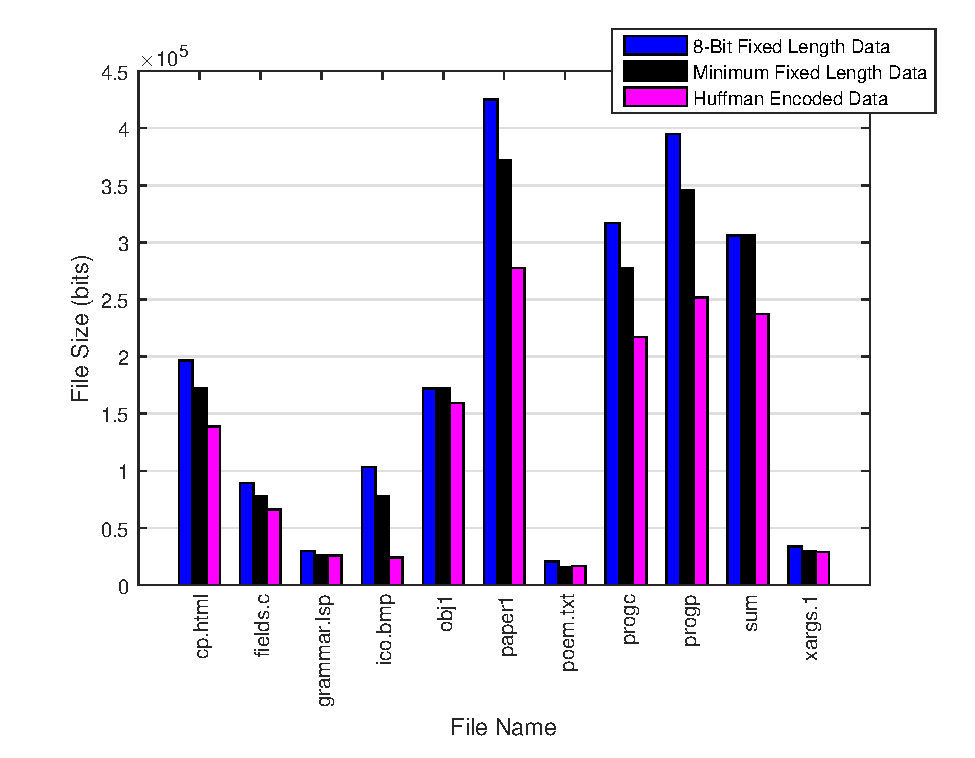
\includegraphics[width=\textwidth]{min_8bit_huffman_size}
	\caption{8-bit Codes vs. Minimum Codes vs. Encoded Huffman Data [File Sizes]}
	\label{fig:8bit_min_encoded_huffman}
\end{figure}

\subsection{LZ4 Encoder}
The following pseudo-code describes how the compression levels for my LZ4 encoder are calculated.
\\\textbf{Compression Evaluation Pseudo-Code:}
\begin{minted}[frame=single, breaklines]{octave}
Obtain the file size of the original file;
Obtain the file size of the compressed binary LZ4 file;

%This gives the compression as a percentage of the original file size
Compression = (compressed_size/ original_file_size)*100

\end{minted}

I have evaluated the compression on a variety of test files as seen below. The below tables (Tables \ref{lz4_enc_results128} - \ref{lz4_enc_results4096}) show the results of my LZ4 encoder. \emph{Note: I have limited the search buffer to 128, 256, 512, 1024, 2048 and 4096 bytes in length respectively.}

For each search buffer size, there is only one file that does not become effectively compressed using this paper's LZ4 encoder implementation (Section \ref{sec_lz4_encoder}), this is `a0020.txt'. Due to the requirements of the LZ4 specification, each compliant LZ4 file must begin with a series of 11 bytes (for specifying options) and must end with four zero bytes; it is due to this, that the compressed `a0020.txt' file becomes large. Only 5 bytes remain to be filled before the encoded size to be as large as the original size.

For the files `a0020.txt' and `a0270.txt', the compression percentages are the same for all search buffer sizes tested. This will often be the case with files consisting of only 1 symbol, on the basis that the match closest to the look-ahead window will always be chosen to be part of the LZ4 data.

As the search buffer is increased, each file either maintains its compression rate, or its compression rate is improved. Taking `xargs.1' as an example. For a search buffer of 128 bytes in length, the test file is compressed to 83.84\% of its original size. Increasing the buffer length up to 4096 bytes, the compression percentage for `xargs.1' becomes 58.39\%. Although the compression improves on increasing the search window size, the runtime also increases. For `xargs.1', the runtime increases from 2.10 seconds (128 byte search buffer), to 15.56 seconds (4096 byte search buffer). Perhaps this seems insignificant, however for some of the other test files, for example `obj1', the respective runtimes are 949.11 seconds (approximately 16 minutes) for a 128 byte search buffer and 3390.79 seconds (approximately $56\frac{1}{2}$ minutes) for a 4096 byte search buffer. This is one possible undesirable factor of this paper's implementation that can be improved with extra work.

Unlike the Huffman encoded data, the test file's original sizes do not directly correspond to the runtime of the algorithm. In circumstances where the LZ4 encoder searches every previous value contained in the search buffer for a match, this may be the case, however I have optimised my LZ4 encoder to only search within the range of the buffer where matched values have been seen before with 100\% certainty.


\begin{table}[H]
	\centering
	\begin{tabular}{| c | c | c | c | c |} 
		\hline
		File-Name & Original Size (bytes) & Encoded Size (bytes) & Runtime(s) & Compression\\
		\hline
		a0020.txt & 20 & 23 & 0.03 & 115.00\%\\
		\hline
		a0270.txt & 270 & 24 & 23.85 & 8.89\%\\
		\hline
		cp.html & 24603 & 20347 & 10.59 & 82.70\%\\
		\hline
		fields.c & 11150 & 7580 & 7.52 & 67.98\%\\
		\hline
		grammar.lsp & 3721 & 2198 & 2.57 & 59.07\%\\
		\hline
		ico.bmp & 12918 & 1383 & 157.25 & 10.71\%\\
		\hline
		obj1 & 21504 & 15282 & 949.11 & 71.07\%\\
		\hline
		paper1 & 53161 & 46979 & 34.03 & 88.37\%\\
		\hline
		poem.txt & 2578 & 2323 & 1.40 & 90.11\%\\
		\hline
		progc & 39611 & 31206 & 25.86 & 78.78\%\\
		\hline
		progp & 49379 & 34136 & 50.16 & 69.13\%\\
		\hline
		sum & 38240 & 26615 & 67.50 & 69.60\%\\
		\hline
		xargs.1 & 4227 & 3544 & 2.10 & 83.84\%\\
		\Xhline{3\arrayrulewidth}
		\textbf{Median} & & & \textbf{23.85} & \textbf{71.07\%}\\
		\hline
	\end{tabular}
	\caption{LZ4 Encoder Compression Results [128 byte search buffer]}
	\label{lz4_enc_results128}
\end{table}

\begin{table}[H]
	\centering
	\begin{tabular}{| c | c | c | c | c |} 
		\hline
		File-Name & Original Size (bytes) & Encoded Size (bytes) & Runtime(s) & Compression\\
		\hline
		a0020.txt & 20 & 23 & 0.02 & 115.00\%\\
		\hline
		a0270.txt & 270 & 24 & 25.91 & 8.89\%\\
		\hline
		cp.html & 24603 & 16728 & 14.57 & 67.99\%\\
		\hline
		fields.c & 11150 & 6773 & 10.51 & 60.74\%\\
		\hline
		grammar.lsp & 3721 & 2058 & 3.80 & 55.31\%\\
		\hline
		ico.bmp & 12918 & 1376 & 292.62 & 10.65\%\\
		\hline
		obj1 & 21504 & 14347 & 1575.32 & 66.72\%\\
		\hline
		paper1 & 53161 & 43411 & 47.03 & 81.66\%\\
		\hline
		poem.txt & 2578 & 2203 & 2.19 & 85.45\%\\
		\hline
		progc & 39611 & 28605 & 36.54 & 72.21\%\\
		\hline
		progp & 49379 & 30260 & 81.88 & 61.28\%\\
		\hline
		sum & 38240 & 25409 & 109.55 & 66.45\%\\
		\hline
		xargs.1 & 4227 & 3299 & 2.89 & 78.05\%\\
		\Xhline{3\arrayrulewidth}
		\textbf{Median} & & & \textbf{25.91} & \textbf{66.72\%}\\
		\hline
	\end{tabular}
	\caption{LZ4 Encoder Compression Results [256 byte search buffer]}
	\label{lz4_enc_results256}
\end{table}

\begin{table}[H]
	\centering
	\begin{tabular}{| c | c | c | c | c |} 
		\hline
		File-Name & Original Size (bytes) & Encoded Size (bytes) & Runtime(s) & Compression\\
		\hline
		a0020.txt & 20 & 23 & 0.02 & 115.00\%\\
		\hline
		a0270.txt & 270 & 24 & 27.84 & 8.89\%\\
		\hline
		cp.html & 24603 & 15477 & 25.15 & 62.91\%\\
		\hline
		fields.c & 11150 & 6134 & 18.57 & 55.01\%\\
		\hline
		grammar.lsp & 3721 & 1893 & 6.71 & 50.87\%\\
		\hline
		ico.bmp & 12918 & 1344 & 565.53 & 10.40\%\\
		\hline
		obj1 & 21504 & 13685 & 2546.57 & 63.64\%\\
		\hline
		paper1 & 53161 & 39617 & 79.25 & 74.52\%\\
		\hline
		poem.txt & 2578 & 2080 & 3.78 & 80.68\%\\
		\hline
		progc & 39611 & 26519 & 61.42 & 66.95\%\\
		\hline
		progp & 49379 & 27299 & 141.60 & 55.28\%\\
		\hline
		sum & 38240 & 24181 & 204.20 & 63.23\%\\
		\hline
		xargs.1 & 4227 & 2998 & 5.09 & 70.93\%\\
		\Xhline{3\arrayrulewidth}
		\textbf{Median} & & & \textbf{27.84} & \textbf{63.23\%}\\
		\hline
	\end{tabular}
	\caption{LZ4 Encoder Compression Results [512 byte search buffer]}
	\label{lz4_enc_results512}
\end{table}

\begin{table}[H]
	\centering
	\begin{tabular}{| c | c | c | c | c |} 
		\hline
		File-Name & Original Size (bytes) & Encoded Size (bytes) & Runtime(s) & Compression\\
		\hline
		a0020.txt & 20 & 23 & 0.02 & 115.00\%\\
		\hline
		a0270.txt & 270 & 24 & 27.22 & 8.89\%\\
		\hline
		cp.html & 24603 & 14266 & 41.50 & 57.98\%\\
		\hline
		fields.c & 11150 & 5444 & 30.83 & 48.83\%\\
		\hline
		grammar.lsp & 3721 & 1843 & 10.30 & 49.53\%\\
		\hline
		ico.bmp & 12918 & 1342 & 973.34 & 10.39\%\\
		\hline
		obj1 & 21504 & 13194 & 2998.94 & 61.36\%\\
		\hline
		paper1 & 53161 & 35962 & 125.44 & 67.65\%\\
		\hline
		poem.txt & 2578 & 1959 & 5.70 & 75.99\%\\
		\hline
		progc & 39611 & 24317 & 94.79 & 61.39\%\\
		\hline
		progp & 49379 & 23500 & 236.01 & 47.59\%\\
		\hline
		sum & 38240 & 22737 & 335.30 & 59.46\%\\
		\hline
		xargs.1 & 4227 & 2740 & 7.81 & 64.82\%\\
		\Xhline{3\arrayrulewidth}
		\textbf{Median} & & & \textbf{41.50} & \textbf{59.46\%}\\
		\hline
	\end{tabular}
	\caption{LZ4 Encoder Compression Results [1024 byte search buffer]}
	\label{lz4_enc_results1024}
\end{table}

\begin{table}[H]
	\centering
	\begin{tabular}{| c | c | c | c | c |} 
		\hline
		File-Name & Original Size (bytes) & Encoded Size (bytes) & Runtime(s) & Compression\\
		\hline
		a0020.txt & 20 & 23 & 0.07 & 115.00\%\\\hline
		a0270.txt & 270 & 24 & 26.40 & 8.89\%\\\hline
		cp.html & 24603 & 13164 & 72.38 & 53.51\%\\\hline
		fields.c & 11150 & 4849 & 53.11 & 43.49\%\\\hline
		grammar.lsp & 3721 & 1774 & 16.66 & 47.68\%\\\hline
		ico.bmp & 12918 & 1333 & 1568.82 & 10.32\%\\\hline
		obj1 & 21504 & 12938 & 3145.90 & 60.17\%\\\hline
		paper1 & 53161 & 32612 & 220.35 & 61.35\%\\\hline
		poem.txt & 2578 & 1903 & 8.07 & 73.82\%\\\hline
		progc & 39611 & 22589 & 164.17 & 57.03\%\\\hline
		progp & 49379 & 20546 & 415.53 & 41.61\%\\\hline
		sum & 38240 & 20998 & 559.22 & 54.91\%\\\hline
		xargs.1 & 4227 & 2571 & 12.25 & 60.82\%\\
		\Xhline{3\arrayrulewidth}
		\textbf{Median} & & & \textbf{72.38} & \textbf{54.91\%}\\
		\hline
	\end{tabular}
	\caption{LZ4 Encoder Compression Results [2048 byte search buffer]}
	\label{lz4_enc_results2048}
\end{table}

\begin{table}[H]
	\centering
	\begin{tabular}{| c | c | c | c | c |} 
		\hline
		File-Name & Original Size (bytes) & Encoded Size (bytes) & Runtime(s) & Compression\\
		\hline
		a0020.txt & 20 & 23 & 0.02 & 115.00\%\\\hline
		a0270.txt & 270 & 24 & 25.77 & 8.89\%\\\hline
		cp.html & 24603 & 12315 & 128.44 & 50.05\%\\\hline
		fields.c & 11150 & 4518 & 87.22 & 40.52\%\\\hline
		grammar.lsp & 3721 & 1771 & 19.30 & 47.59\%\\\hline
		ico.bmp & 12918 & 1273 & 2614.69 & 9.85\%\\\hline
		obj1 & 21504 & 12706 & 3390.79 & 59.09\%\\\hline
		paper1 & 53161 & 29556 & 402.78 & 55.60\%\\\hline
		poem.txt & 2578 & 1895 & 8.23 & 73.51\%\\\hline
		progc & 39611 & 20766 & 295.83 & 52.42\%\\\hline
		progp & 49379 & 17268 & 723.49 & 34.97\%\\\hline
		sum & 38240 & 20291 & 977.55 & 53.06\%\\\hline
		xargs.1 & 4227 & 2468 & 15.56 & 58.39\%\\
		\Xhline{3\arrayrulewidth}
		\textbf{Median} & & & \textbf{128.44} & \textbf{52.42\%}\\
		\hline
	\end{tabular}
	\caption{LZ4 Encoder Compression Results [4096 byte search buffer]}
	\label{lz4_enc_results4096}
\end{table}

\subsection{Huffman Encoder vs. LZ4 Encoder}
This section analyses the performance of the presented Huffman encoder (Section \ref{sec_huff_enc}) and LZ4 encoder implementations (Section \ref{sec_lz4_encoder}). Figure \ref{fig:lz4_compression} below shows a grouped bar chart with the compression percentage of each file (excluding `a0020.txt' and `a0270.txt') for LZ4 encoded data (128 byte buffer - 4096 byte buffer) and Huffman encoded data. The compression rate for Huffman data is based on the original file being encoded using an 8-bit fixed-length system. 

From the graph, we can deduce that LZ4 compression tends to exceed Huffman compression, with a few exceptions. In some cases, such as for `progc', Huffman encoding compresses the original data better than LZ4 encoding with search buffers of 128 bytes and 256 bytes, however LZ4 surpasses the Huffman value when the search buffer is set to 512 bytes to 4096 bytes in length. The file `paper1' is interesting, as even for a search buffer of 1024 bytes in length, Huffman encoding produces a better compression value than LZ4. However, by increasing the search buffer to 2048 to 4096 bytes, LZ4 does finally surpass the Huffman encoding implementation.

Again, `a0020.txt' proves to provide seemingly anomalous data, however after previous analysis, we know that due to the requirements of the LZ4 specification, the encoded LZ4 file size is large in comparison to the Huffman encoded file.

\begin{figure}[H]
	\centering
	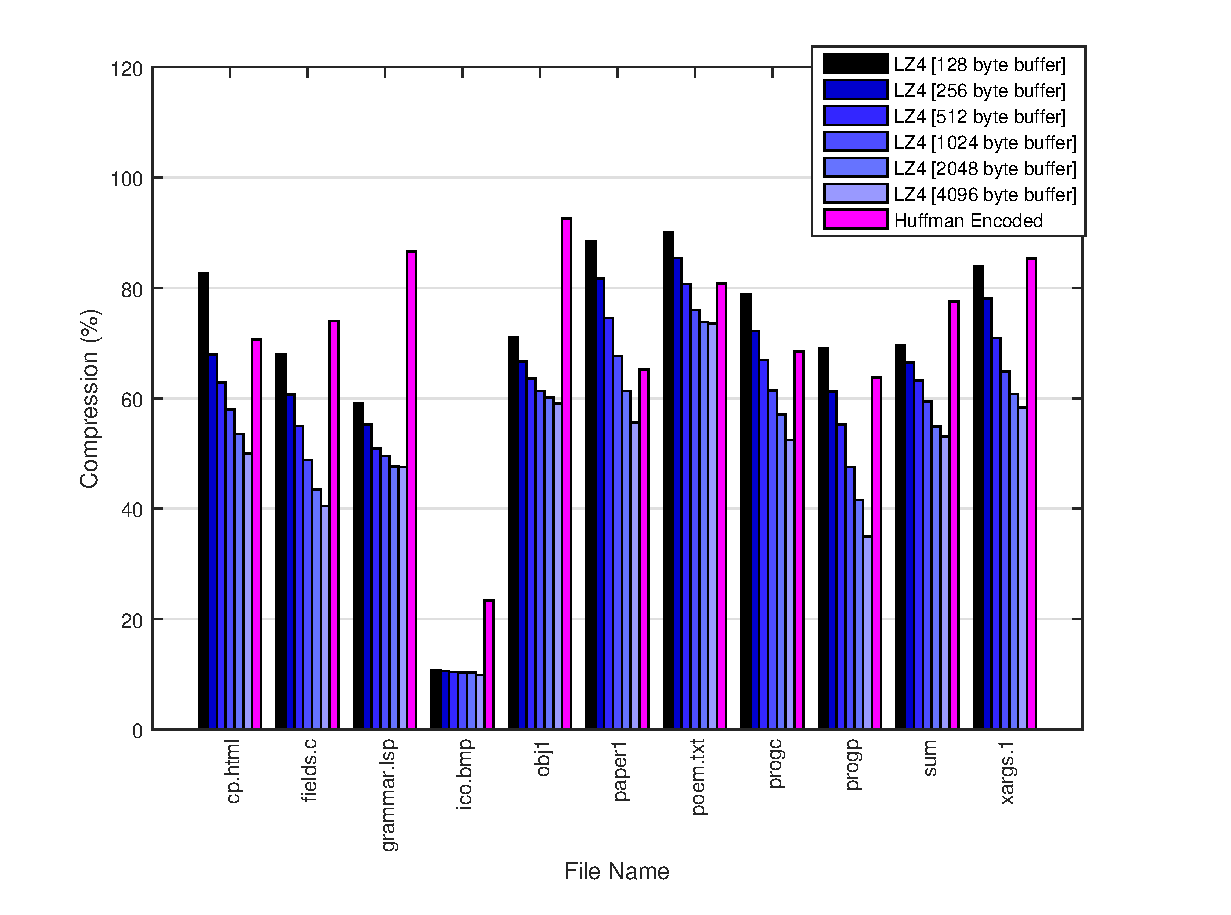
\includegraphics[width=\textwidth]{lz4_compression}
	\caption{LZ4 Encoder [128-4096 byte buffer] vs Huffman Encoder Compression}
	\label{fig:lz4_compression}
\end{figure}

\clearpage
Overall for the compressor implementations as outlined in this paper, LZ4 appears to be able to perform best on a number of files with varying content; however this is dependant on the size of the search buffer. Figure \ref{fig:average_compression} below shows that each of my implementations, on average, compress to approximately 70\% - this fulfils my second objective in Section \ref{sec_objectives}. Of course, to make this test fairer, more files would have to be tested, however for my sample, this is true. The graph demonstrates that as the search buffer is increased, it is likely that the compression value for this LZ4 implementation will improve. 

It appears that Huffman, on average performs slightly better ($70.62\%$) than LZ4 with a 128 byte search buffer ($71.07\%$), however when the buffer is increased to 256, 512, 1024, 2048 and 4096 bytes, LZ4 surpasses the average compression value of Huffman ($66.42\%$, $63.23\%$, $59.46\%$, $54.91\%$ and $52.42\%$ respectively). 

\begin{figure}[H]
	\centering
	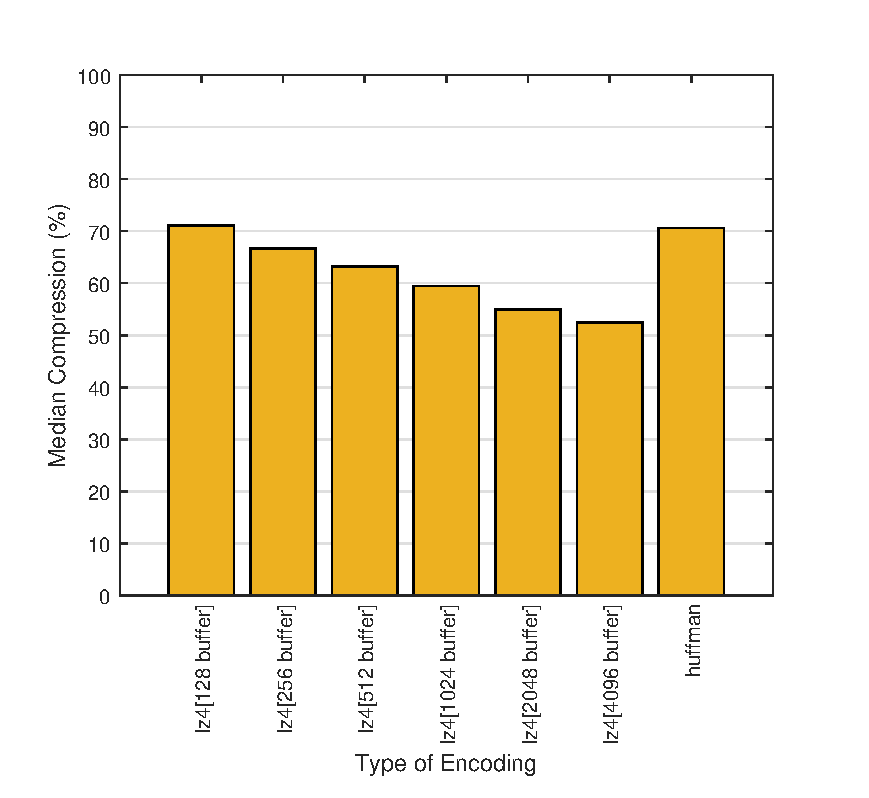
\includegraphics[width=6.0in]{average_compression}
	\caption{Average LZ4 vs Huffman Encoder Compression}
	\label{fig:average_compression}
\end{figure}

Although Figure \ref{fig:average_compression} shows the median compression for each compressor implementation, one factor that isn't considered is the runtime of each encoder. Figure \ref{fig:average_runtime} displays the runtime of the Huffman and LZ4 encoders.

Below, the graph shows us that the runtime for Huffman ($14.44s$) is faster than any of the LZ4 implementations (the next fastest being LZ4 with a 128 byte search buffer at $23.85s$ on average). Considering the tested files are of 64KB in size or less, the runtimes appear to be very large. With more time and effort, runtimes could likely be improved significantly.

Comparing Figure \ref{fig:average_runtime} with Figure \ref{fig:average_compression}, it seems that LZ4 with a 128 byte search buffer is almost never desired due to Huffman surpassing it in both average compression and average runtime. If time is no object, LZ4 with a 4096 byte search buffer is the most desirable of the tested implementations due to the average compression being better than it's competitors. As increasing the search buffer will not make the compression worse for an LZ4 encoder, the user may wish to alter the search window to search all previous values; this will ensure the best possible compression for this LZ4 encoder, however the runtime may be significantly increased dependant on the file size and the number of matches found.

\begin{figure}[H]
	\centering
	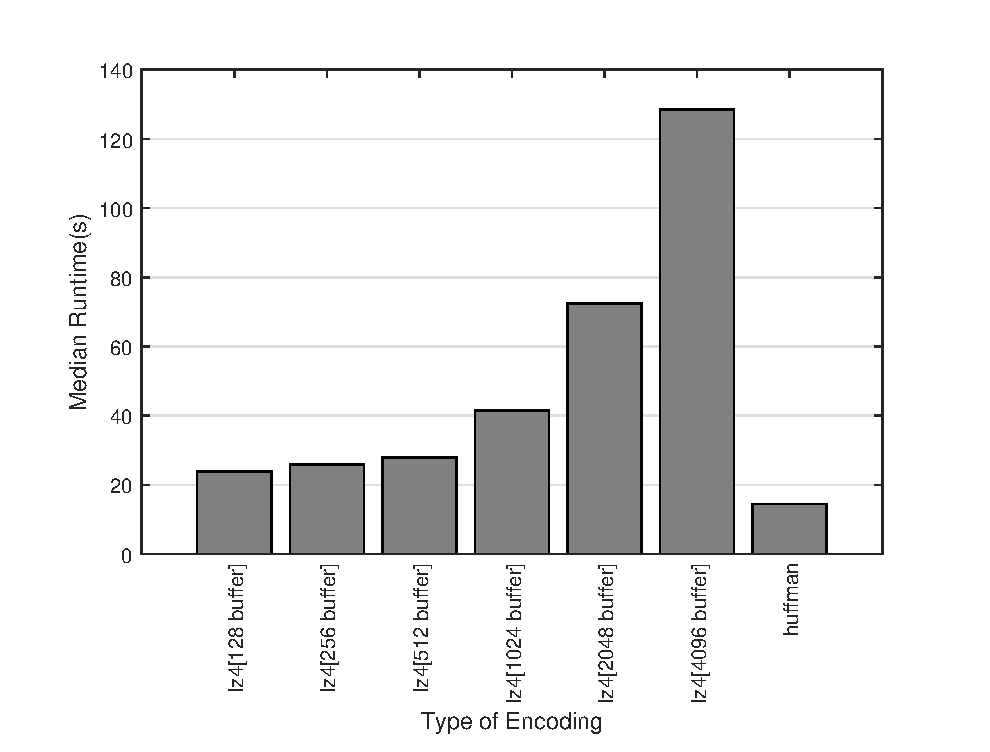
\includegraphics[width=6.0in]{average_runtime}
	\caption{Average LZ4 vs Huffman Encoder Runtime}
	\label{fig:average_runtime}
\end{figure}
\clearpage

\subsection{Commercial Compressor Comparison}
There are a variety of compressors available commercially and for personal use. This section shall compare my compressor implementation results with those of some commercial and open-source compressors.

The commercial compressors I have chosen to compare my results to, are:
\begin{itemize}
	\item \textbf{smalLZ4} - an optimal LZ4 compressor\footnote{http://create.stephan-brumme.com/smallz4/};
	\item \textbf{WinRAR} - a popular, powerful archive manager\footnote{https://www.rarlab.com/};
	\item \textbf{7-Zip} - a tool known for its high compression ratio\footnote{http://www.7-zip.org/}.
\end{itemize}

I have chosen smalLZ4 as this aligns with my LZ4 implementation, WinRAR as this is a popular tool with many users and 7-Zip because its compression level is known to be high.

\subsubsection{SmalLZ4}
SmalLZ4 performs optimal compression by default. Optimal here means that smalLZ4 has been proven to be impossible to surpass in compression rate when compared to another LZ4 compliant encoder. I shall perform three tests with smallz4, one for optimal compression (flag -9), one for least compression without being uncompressed (flag -1) and another for mid-range compression (flag -4).

I shall be using the Windows executable `smallz4-v1.0.exe' available from the smallz4 website. To compress the specified files, the commands run in `windows command prompt' are:

\begin{minted}[frame=single, breaklines]{text}
%the flag will be changed to 1, 4 and 9 for each file
smallz4-v1.0.exe -<flag> <filename>.<extenion> <filename>.lz4
\end{minted}

The results after compressing each file is as 
below in Table \ref{smallz4_results_size} and Table \ref{smallz4_results_compression}.

\begin{table}[H]
	\centering
	\begin{tabular}{| c | c | c | c | c |} 
		\hline
		File-Name & Original Size & smalLZ4 -1 & smalLZ4 -4 & smalLZ4 -9 \\
		& (bytes) & (bytes) & (bytes) & (bytes) \\
		\hline
		a0020.txt & 20 & 25 & 25 & 25\\
		\hline
		a0270.txt & 270 & 26 & 26 & 26\\
		\hline
		cp.html & 24603 & 15228 & 13229 & 10306\\
		\hline
		fields.c & 11150 & 7087 & 5767 & 4217\\
		\hline
		grammar.lsp & 3721 & 2579 & 2213 & 1733\\
		\hline
		ico.bmp & 12918 & 7111 & 1885 & 1063\\
		\hline
		obj1 & 21504 & 15147 & 14631 & 12362\\
		\hline
		paper1 & 53161 & 36613 & 30970 & 23043\\
		\hline
		poem.txt & 2578 & 2305 & 2216 & 1867\\
		\hline
		progc & 39611 & 26619 & 23067 & 17172\\
		\hline
		progp & 49379 & 27399 & 20014 & 14246\\
		\hline
		sum & 38240 & 23750 & 21298 & 16304\\
		\hline
		xargs.1 & 4227 & 3221 & 2992 & 2416\\
		\hline
	\end{tabular}
	\caption{SmalLZ4 Encoder Size Results}
	\label{smallz4_results_size}
\end{table}

\emph{Remark: `smalLZ4 -9' is optimal LZ4 encoding, however for `a0020.txt' and `a0270.txt', the number of bytes is larger than that of my implementation. The reason for this is because my implementation does not follow the LZ4 specification specifically. SmalLZ4 implements the requirement of having 5 uncompressed bytes at the end of the LZ4 data, where my implementation does not.}

\begin{table}[H]
	\centering
	\begin{tabular}{| c | c | c | c | c |} 
		\hline
		File-Name & Original Size & smalLZ4 -1 & smalLZ4 -4 & smalLZ4 -9 \\
		& (bytes) & Compression & Compression & Compression\\
		\hline
		a0020.txt & 20 & 125.00\% & 125.00\% & 125.00\%\\
		\hline
		a0270.txt & 270 & 9.63\% & 9.63\% & 9.63\%\\
		\hline
		cp.html & 24603 & 61.89\% & 53.77\% & 41.89\%\\
		\hline
		fields.c & 11150 & 63.56\% & 51.72\% & 37.82\%\\
		\hline
		grammar.lsp & 3721 & 69.31\% & 59.47\% & 46.57\%\\
		\hline
		ico.bmp & 12918 & 55.05\% & 14.59\% & 8.83\%\\
		\hline
		obj1 & 21504 & 70.44\% & 68.04\% & 57.49\%\\
		\hline
		paper1 & 53161 & 68.87\% & 58.26\% & 43.35\%\\
		\hline
		poem.txt & 2578 & 89.41\% & 85.96\% & 72.42\%\\
		\hline
		progc & 39611 & 67.20\% & 58.23\% & 43.35\%\\
		\hline
		progp & 49379 & 55.49\% & 40.53\% & 28.85\%\\
		\hline
		sum & 38240 & 62.11\% & 55.70\% & 42.64\%\\
		\hline
		xargs.1 & 4227 & 76.20\% & 70.78\% & 57.16\%\\
		\Xhline{3\arrayrulewidth}
		\textbf{Median} & & \textbf{67.20\%} & \textbf{58.23\%} & \textbf{43.35\%}\\
		\hline
	\end{tabular}
	\caption{SmalLZ4 Encoder Compression Results}
	\label{smallz4_results_compression}
\end{table}

\subsubsection{WinRAR}
Similarly to smalLZ4, this section will analyse WinRAR at three levels of compression. For WinRAR, the flags I will be using are `-m1' (least compression without being uncompressed), `-m3' (mid-compression) and `-m5' (best compression). I will be using the command line Windows version 5.50 (x64) of WinRAR, available from the official website. I will utilise the following commands for my test files:

\begin{minted}[frame=single, breaklines]{text}
%'a' means 'add to archive'; flags = m1, m3 and m5
rar a -<flag> <filename>-<flag>.rar <filename>.<extension>
\end{minted}

\emph{Remark: When testing the compression of my files, I shall be using the graphical WinRAR interface to check the compressed file sizes. The storage space of the archive itself is often larger than the compressed size of the file due to additional content added to the archive file.}

The below tables (Table \ref{winrar_results_size} and Table \ref{winrar_results_compression}) display the results of the WinRAR compression.

\begin{table}[H]
	\centering
	\begin{tabular}{| c | c | c | c | c |} 
		\hline
		File-Name & Original Size & rar -m1 & rar -m3 & rar -m5 \\
		& (bytes) & (bytes) & (bytes) & (bytes) \\
		\hline
		a0020.txt & 20 & 12 & 12 & 12\\
		\hline
		a0270.txt & 270 & 13 & 13 & 13\\
		\hline
		cp.html & 24603 & 8737 & 7948 & 7946\\
		\hline
		fields.c & 11150 & 3564 & 3096 & 3097\\
		\hline
		grammar.lsp & 3721 & 1317 & 1249 & 1249\\
		\hline
		ico.bmp & 12918 & 883 & 684 & 672\\
		\hline
		obj1 & 21504 & 10543 & 9764 & 9764\\
		\hline
		paper1 & 53161 & 21267 & 18114 & 18107\\
		\hline
		poem.txt & 2578 & 1321 & 1283 & 1283\\
		\hline
		progc & 39611 & 15018 & 13137 & 13128\\
		\hline
		progp & 49379 & 12844 & 10733 & 10724\\
		\hline
		sum & 38240 & 13629 & 11483 & 11483\\
		\hline
		xargs.1 & 4227 & 1860 & 1759 & 1759\\
		\hline
	\end{tabular}
	\caption{WinRAR Encoder Size Results}
	\label{winrar_results_size}
\end{table}

\begin{table}[H]
	\centering
	\begin{tabular}{| c | c | c | c | c |} 
		\hline
		File-Name & Original Size & rar -m1 & rar -m3 & rar -m5 \\
		& (bytes) & Compression & Compression & Compression\\
		\hline
		a0020.txt & 20 & 60.00\% & 60.00\% & 60.00\%\\
		\hline
		a0270.txt & 270 & 4.81\% & 4.81\% & 4.81\%\\
		\hline
		cp.html & 24603 & 35.51\% & 32.31\% & 32.30\%\\
		\hline
		fields.c & 11150 & 31.96\% & 27.77\% & 27.78\%\\
		\hline
		grammar.lsp & 3721 & 35.39\% & 33.57\% & 33.57\%\\
		\hline
		ico.bmp & 12918 & 6.84\% & 5.29\% & 5.20\%\\
		\hline
		obj1 & 21504 & 49.03\% & 45.41\% & 45.41\%\\
		\hline
		paper1 & 53161 & 40.00\% & 34.07\% & 34.06\%\\
		\hline
		poem.txt & 2578 & 51.24\% & 49.77\% & 49.77\%\\
		\hline
		progc & 39611 & 37.91\% & 33.17\% & 33.14\%\\
		\hline
		progp & 49379 & 26.01\% & 21.74\% & 21.72\%\\
		\hline
		sum & 38240 & 35.64\% & 30.03\% & 30.03\%\\
		\hline
		xargs.1 & 4227 & 44.00\% & 41.61\% & 41.61\%\\
		\Xhline{3\arrayrulewidth}
		\textbf{Median} & & \textbf{35.64\%} & \textbf{33.17\%} & \textbf{33.14\%}\\
		\hline
	\end{tabular}
	\caption{WinRAR Encoder Compression Results}
	\label{winrar_results_compression}
\end{table}

\subsubsection{7-Zip}
For 7-Zip, I have chosen to analyse the compression rates when the flags are set to `-mx1' (least compression) and `-mx9' (best compression). After performing some tests on intermediate compression levels, I discovered that almost no change (if any) was found, therefore I have kept to the extremes.

Once again, I shall be running these tests using the the Windows command line version of 7-Zip (version 18.01 x64). The commands to be run are as follows:

\begin{minted}[frame=single, breaklines]{text}
%'a' means 'add to archive'; flags = mx1 and mx9
7z a -<flag> <filename>-<flag>.7z <filename>.<extension>
\end{minted}

The results of 7-Zip compression on the test files are stored in the tables below (Table \ref{7z_results_size} and Table \ref{7z_results_compression}).

\begin{table}[H]
	\centering
	\begin{tabular}{| c | c | c | c |} 
		\hline
		File-Name & Original Size & 7z -mx1 & 7z -mx9\\
		& (bytes) & (bytes) & (bytes) \\
		\hline
		a0020.txt & 20 & 14 & 14\\
		\hline
		a0270.txt & 270 & 14 & 14\\
		\hline
		cp.html & 24603 & 7993 & 7589\\
		\hline
		fields.c & 11150 & 3128 & 2978\\
		\hline
		grammar.lsp & 3721 & 1273 & 1236\\
		\hline
		ico.bmp & 12918 & 701 & 657\\
		\hline
		obj1 & 21504 & 9549 & 9371\\
		\hline
		paper1 & 53161 & 18179 & 17220\\
		\hline
		poem.txt & 2578 & 1336 & 1306\\
		\hline
		progc & 39611 & 13128 & 12501\\
		\hline
		progp & 49379 & 10965 & 10303\\
		\hline
		sum & 38240 & 10231 & 9415\\
		\hline
		xargs.1 & 4227 & 1801 & 1755\\
		\hline
	\end{tabular}
	\caption{7-Zip Encoder Size Results}
	\label{7z_results_size}
\end{table}

\begin{table}[H]
	\centering
	\begin{tabular}{| c | c | c | c |} 
		\hline
		File-Name & Original Size & 7z -mx1 & 7z -mx9\\
		& (bytes) & Compression & Compression\\
		\hline
		a0020.txt & 20 & 70.00\% & 70.00\%\\
		\hline
		a0270.txt & 270 & 5.19\% & 5.19\%\\
		\hline
		cp.html & 24603 & 32.49\% & 30.85\%\\
		\hline
		fields.c & 11150 & 28.05\% & 26.71\%\\
		\hline
		grammar.lsp & 3721 & 34.21\% & 33.22\%\\
		\hline
		ico.bmp & 12918 & 5.43\% & 5.09\%\\
		\hline
		obj1 & 21504 & 44.41\% & 43.58\%\\
		\hline
		paper1 & 53161 & 34.20\% & 32.39\%\\
		\hline
		poem.txt & 2578 & 51.82\% & 50.66\%\\
		\hline
		progc & 39611 & 33.14\% & 31.56\%\\
		\hline
		progp & 49379 & 22.21\% & 20.87\%\\
		\hline
		sum & 38240 & 26.75\% & 24.62\%\\
		\hline
		xargs.1 & 4227 & 42.61\% & 41.52\%\\
		\Xhline{3\arrayrulewidth}
		\textbf{Median} & & \textbf{33.14\%} & \textbf{31.56\%}\\
		\hline
	\end{tabular}
	\caption{7-Zip Encoder Compression Results}
	\label{7z_results_compression}
\end{table}

\subsubsection{Graphical Comparison}
After evaluating the compression percentages for various commercial/open-source compressors, this section displays a graph of the average rate of compression for each, to see how the compressors outlined in this paper compare.

Figure \ref{fig:commercial_comparison} below displays the difference in average compression between my implemented compressors and some commercial and open-source compressors. Overall, with my implemented LZ4 compressor with a 2048 and 4096 byte search buffer, I have managed to perform better than smalLZ4 at its mid-range compression level. My implementation of LZ4 may be able to near that of smalLZ4 at the optimal compression level if the search buffer is increased. It is clear that with an increasing search buffer, my implementation of LZ4 grows nearer to the optimal value.

Each implementation in this paper, except for LZ4 with a 128 byte search buffer, surpasses smalLZ4 at its lowest level of compression, however none of the WinRAR or 7-Zip compression values have been reached. As smalLZ4 is optimal LZ4 compression, the WinRAR and 7-Zip compression levels cannot be matched for the test files using LZ4 encoding.

Although my implementations appear to have performed reasonably well, there is still the issue of runtime to address. I have not included a runtime graph comparison, as each of the commercial/open source compressor's runtimes on each file did not exceed 1 second. This proves that there is still work to be done with my implementations.

\begin{figure}[H]
	\centering
	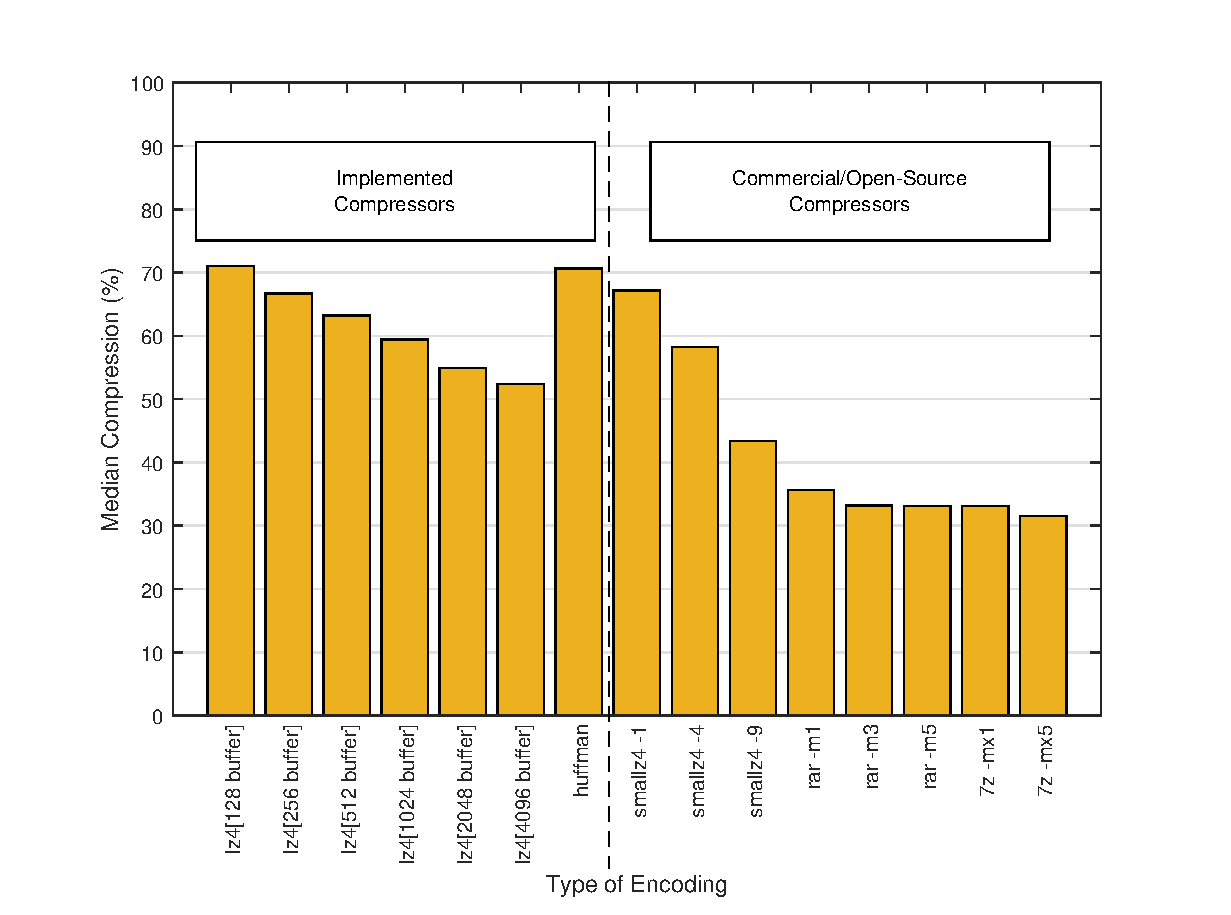
\includegraphics[width=\textwidth]{commercial_comparison}
	\caption{Implementation vs. Commercial Encoder Compression}
	\label{fig:commercial_comparison}
\end{figure}

\subsection{Decompresser Implementations}
As previously discussed in Sections \ref{sec_huff_decoder} and \ref{sec_lz4_encoder}, I have developed implementations of decoders for LZ4 and Huffman encoded data. These both served to be extremely useful during debugging of my encoders; they helped me verify that my encoded data was compliant with the appropriate encoding specifications.

Each decompresser works as expected, however I shall analyse their runtimes in comparison to each other. See Table \ref{decoder_runtimes} below for the evaluated runtimes of my decoders on each test file.

\begin{table}[H]
	\centering
	\begin{tabular}{| c | c | c |} 
		\hline
		File-Name & Huffman Decoder & LZ4 Decoder\\
		& Runtime(s) & Runtime(s)\\
		\hline
		a0020.txt & 0.01 & 0.003\\
		\hline
		a0270.txt & 0.07 & 0.01\\
		\hline
		cp.html & 17.90 & 12.81\\
		\hline
		fields.c & 7.76 & 3.17\\
		\hline
		grammar.lsp & 2.20 & 0.55\\
		\hline
		ico.bmp & 3.25 & 3.59\\
		\hline
		obj1 & 33.74 & 9.51\\
		\hline
		paper1 & 34.24 & 57.07\\
		\hline
		poem.txt & 1.33 & 0.38\\
		\hline
		progc & 30.31 & 32.41\\
		\hline
		progp & 32.29 & 49.08\\
		\hline
		sum & 42.10 & 29.59\\
		\hline
		xargs.1 & 2.70 & 0.74\\
		\Xhline{3\arrayrulewidth}
		\textbf{Median} & \textbf{7.76} & \textbf{3.59}\\
		\hline
	\end{tabular}
	\caption{Implemented Decoder Runtime Results}
	\label{decoder_runtimes}
\end{table}

The below Figures \ref{fig:decoder_file_time} and \ref{fig:decoder_average_time}, show a per-file and median comparison (respectively) of the decompression time for the encoded test files (once again excluding `a0020.txt' and `a0270.txt' in the former case). 

The runtime for Huffman is slower than that of LZ4, this is likely due to using string processing. There are multiple occasions where the LZ4 decoder performs faster than the Huffman decoder, however, there are also multiple instances of the opposite case. For the test files, the LZ4 decoder completes decoding in approximately half the time of Huffman.

Currently, my Huffman decoder uses two text files in combination to produce an output file, this could be inefficient. If I were able to enhance my implementation by producing a Huffman encoder and decoder that works with just one binary file consisting of the dictionary and the encoded data, there is potential the Huffman decoder may perform better than the current version of the LZ4 decoder.

\begin{figure}[H]
	\centering
	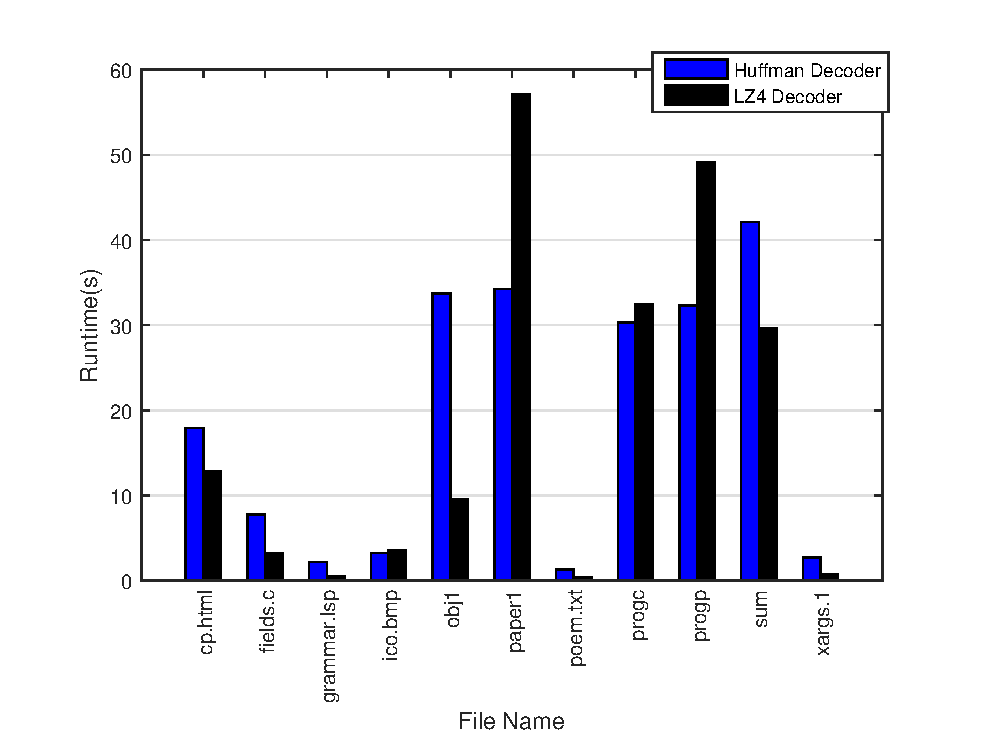
\includegraphics[width=6.0in]{decoder_file_time}
	\caption{Decoder Runtime for Test Files}
	\label{fig:decoder_file_time}
	\setlength{\floatsep}{0pt}
\end{figure}
\begin{figure}[H]
	\centering
	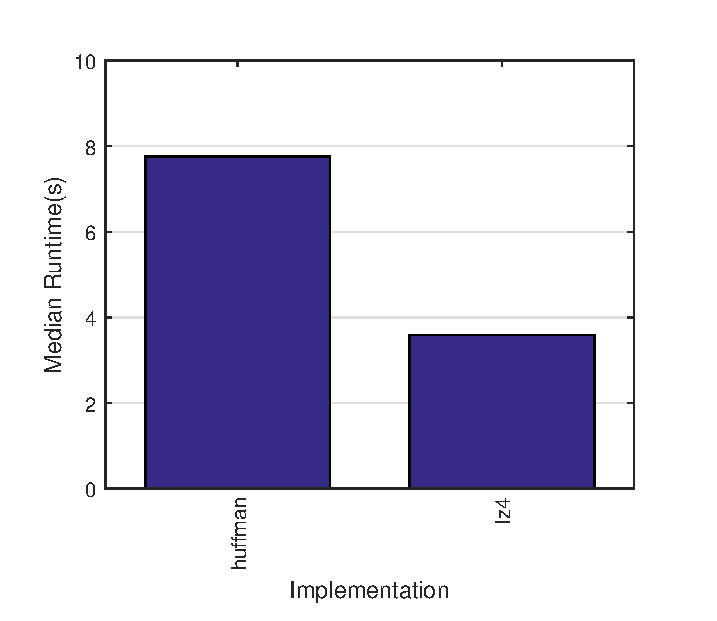
\includegraphics[trim={0 0 0 1cm}, width=4.5in]{decoder_average_time}
	\caption{Median Decoder Runtime for Test Files}
	\label{fig:decoder_average_time}
\end{figure}

\section{Conclusion and Recommendations}
\subsection{Objective Achievements}
At the beginning of this paper, I set out a number of objectives. Recapitulating, these were:

\begin{enumerate}
	\item Produce two working data compressors;
	\item Achieve a good level of compression;
	\item Understand the suitability of algorithm types;
	\item Deliver a high-quality, detailed dissertation write-up.
\end{enumerate}

During the course of this dissertation, I have understood a variety of lossless data compression techniques and algorithms, including Huffman Coding, LZ77 and LZ4. Learning where each algorithm is most suitable has been an essential task. For example, for data consisting of a limited number of symbols that is large in size, it is likely that Huffman Coding will be suitable. This is due to each symbol likely being represented by, on average, less bits per symbol than the original system's fixed-length encoding (such as ASCII-8/UTF-16) [\textbf{Objective 3 fulfilled}].

Applying my understanding of various lossless compression techniques, I have successfully been able to produce an encoder and a decoder for two different methods - Huffman Coding and LZ4. My decoders have acted as secondary verification that my encoders work sufficiently. While my LZ4 encoder is not 100\% compliant with the official specification, it does implement some of the additional content required outside of the actual data blocks (such as a beginning verification marker) [\textbf{Objective 1 fulfilled}].

Initially, the compression aim for my encoders was 70\% on average for both. Each of the implementations in this paper have managed to achieve approximately this value. The Huffman encoder has achieved 70.62\% compression on average (compared to an 8-bit fixed length encoding), whereas the LZ4 encoder has reached 52.42\% average compression for a 4096 byte search buffer. My Huffman implementation has managed to encode one of the uncompressed test files (`a0270.txt') to 14.72\% of its original size, while my LZ4 encoder has compressed the same file to 8.89\% of its original size [\textbf{Objective 2 fulfilled}].

For the final objective, I have attempted to keep my quality of writing consistent throughout this paper. Where appropriate, I have explained new concepts in a suitable level of English so that those with a similar knowledge about algorithmic and mathematical methods as myself, should be able to understand them without much difficulty [\textbf{Objective 4 fulfilled}].

\subsection{Conclusion}
There have been many aspects of this research that have been rewarding such as providing myself, and the readers of the paper, with a key understanding of lossless compression techniques and an insight into why they are important. Although this research has not served as a step-by-step guide, it contains a wealth of information to help someone who is new to this concept to produce their own working Huffman, LZ77 or LZ4 compressor(s) and compare their rates of compression and runtimes to those in this paper.

Another positive point of this research, is that the algorithms produced are not programming language specific. If a reader of this research has a good knowledge of any programming language, they should be able to sufficiently produce a number of working encoders and decoders after reading this paper and understanding the addressed algorithms. As the implementations presented are somewhat abstract, there is room for improvement in runtime and potentially rate of compression; the programming language chosen could possibly affect this.

Based on the initial expectations, the encoders produced as supporting material to this project have successfully compressed 13 different test files, each containing differing content and alphabet sizes. The developed Huffman and LZ4 encoders have met the expectations of achieving approximately 70\% compression on average (70.62\% and 52.42\% respectively); due to this, the implemented encoders have been proven to perform comparably to `smalLZ4', an open-source compressor, whilst it provides low to medium compression. Although comparable to smalLZ4, my encoders cannot compete with WinRAR or 7-Zip (providing 33.14\% and 31.56\% compression respectively). This is proven because smalLZ4 with the flag `-9' is optimal LZ4 encoding. 

Considering that `smalLZ4' can provide optimal LZ4 encoding, however good this paper's implementation is, it will not be able to surpass the compression rate of smalLZ4 and therefore cannot beat WinRAR or 7-Zip compression rates on the included set of test files. While not being able to beat or effectively compare to these methods alone, further research could be performed into combining LZ4 with other compression techniques to attempt to reach better compression levels.

While this research has been wholly beneficial as a gateway into understanding lossless compression, there are many improvements to be made, some of which are discussed in the recommendations section below.

\subsection{Recommendations}
This section provides an assortment of recommendations for future work to develop this project further. These recommendations listed in order of implementation and functionality importance (based on my own personal judgement). If I were to implement the following recommendations, I would do so in the order in which they are presented.

\subsubsection{Huffman File Merging}
One recommendation for anyone who intends to improve this research, is to merge the output encoded data and dictionary from the Huffman encoder into one file. To achieve this, it may be easier to store both pieces of data as binary data and append the encoded data after the dictionary data (with a separating marker). The advantages of merging these files are that there will be fewer files, therefore the working directory should be less cluttered. If the encoded data and dictionary are stored as one binary file, the rate of compression for Huffman will improve (currently the dictionary is stored as a series of bytes with an 8-bit fixed length).

\subsubsection{Huffman Binary Decoder}
Once the Huffman encoder is configured to output a binary file (or possibly still two) containing the encoded data and dictionary, the next step is to alter the current Huffman decoder implementation to accept binary values rather than bytes. The purpose of this is to match the decoder with the functionality of the encoder.

\subsubsection{LZ4 Matching Optimisation}
Currently, the implemented encoder takes the best match as being the one with the longest length in the search buffer. While this provides good results, the longest match for a particular set of symbols may not always give the best compression results possible for the data overall. To optimise matching, a future implementation should consider results of previous matches and be aware of possible combinations of future matches in the data. 

An example of where the longest match value is not optimal is displayed for the data `\textbf{aaaaabaacaaa}'. When encoding this using LZ4, the following two encodings are valid (\emph{numeric values are written in decimal}):

\begin{table}[H]
	\centering
	\begin{tabular}{| c | c | c | c | c | c | c | c | c | c | c | c | c | c |} 
		\hline
		Byte:&1&2&3&4&5&6&7&8&9&10&11&12&13\\
		\hline
		Data:&62&a&a&a&a&a&b&03&00&13&c&07&00\\
		\hline
	\end{tabular}
	\caption{Longest Match Encoding}
	\label{encoding_1}
\end{table}

The example data could be represented as per Table \ref{encoding_1} above. This is a valid encoding and is created based on the previously seen values that have the longest match. An LZ4 representation that uses fewer bytes is located in Table \ref{encoding_2}. This representation takes into account other token combinations rather than just the longest match.

\begin{table}[H]
	\centering
	\begin{tabular}{| c | c | c | c | c | c | c | c | c | c | c | c |} 
		\hline
		Byte:&1&2&3&4&5&6&7&8&9&10&11\\
		\hline
		Data:&14&a&01&00&43&b&a&a&c&07&00\\
		\hline
	\end{tabular}
\caption{Optimised Encoding}
	\label{encoding_2}
\end{table}

Further research is required to be able to implement this, however compression results can potentially be improved using this method.

\subsubsection{LZ4 Runtime Efficiency}
As previously concluded, the LZ4 implementation produces good results, however this is at the cost of lengthy runtimes. One way to improve this is to use `hash chains' as noted on the `LZ4 Block Format' page of \citep{lz4_github}. This page also states: ``there is no assumption nor limits to the way to compressor searches and selects matches within the source data block." This shows that the use of hash chains may not be the only way to improve efficiency, there are possibly many solutions.

\subsubsection{Canonical Huffman Codes}
Canonical Huffman Codes are Huffman codes chosen specifically due to their efficient and `simple to use' properties. Codes in canonical form can be identified using just a few parameters (depending on the way they are stored) such as the length of the code, and the code itself. If the symbols are stored in a particular order (for example alphabetically), the dictionary representation may not need to include the actual symbol value, as the order is already predefined \citep[pp.~84-88]{dc_complete_ref}. Use of Canonical Huffman Codes would be beneficial as the dictionary size could be decreased while efficiency of searching could be improved.

\subsubsection{LZ4 Specification Compliance}
One major factor of this research is that the implementation produced is not \emph{true} LZ4. Many seemingly unnecessary and specific artefacts contained within the specification have been omitted, including leaving at least the final 5 bytes of data unencoded. The presented implementation uses an LZ4 algorithmic approach to encode and decode LZ4-like data, however if compared to the specification, it would not be accepted as a true LZ4 implementation. One desirable part of the specification is used to be able to run the LZ4 encoder on more currently `realistic' test files, consisting of sizes exceeding 64KB in size.

\subsubsection{Runtime Analysis}
Currently, the analysis of the average runtime for each algorithm is calculated using the median value. While this provides useful information, perhaps as future work, an analysis of `input/output bytes processed per second' could give a clearer picture of exactly how efficient each encoder and decoder is. This should be fairly simple to implement and plot.

\subsubsection{Compression Method Merging}
While the results for the methods used in this paper have been good, there is the possibility to improve these results further by combining Huffman encoding with LZ4. By doing this, there is future potential perhaps exceed the compression rate of smalLZ4 at its optimal level. Method merging is not confined to the combination of Huffman and LZ4, it may be possible and more beneficial to merge other methods (considered out of scope for this project) with the implementations included in this paper. 

ZIP is popularly used as a tool for compression of files in the public domain. ZIP is an example of a working compression tool that merges different algorithms. The Deflate algorithm used in ZIP is a merging of a style of LZ77 compression combined with Huffman Coding that provides good compression rates in reasonable time \citep[pp.~230-241]{dc_complete_ref}. The Deflate method for compressing data is detailed in RFC 1951\footnote{https://www.ietf.org/rfc/rfc1951.txt}.

\clearpage


\section*{Appendix A}
\subsection*{Table of Test File Information}
\addcontentsline{toc}{section}{Appendix A}
\addcontentsline{toc}{subsection}{Table of Test File Information}
\begin{table}[H]
	\centering
	\hspace*{-0.4cm}\begin{tabular}{| c | c | c | c |} 
		\hline
		\textbf{File-Name} & \textbf{File-Size (bytes)} & \textbf{Description} & \textbf{Source}\\
		\hline
		a0020.txt & 20 & 20 `$a$' symbols & Independent Creation\\
		\hline
		a0270.txt & 270 & 270 `$a$' symbols & Independent Creation\\
		\hline
		cp.html & 24,603 & A sample web page & Canterbury Corpus\\
		\hline
		fields.c & 11,150 & Source code written in C & Canterbury Corpus\\
		\hline
		grammar.lsp & 3,721 & Source code written in LISP & Canterbury Corpus\\
		\hline
		ico.bmp & 12,918 & Black/White/Grey Bitmap Image & Online\tablefootnote{Image found at `https://www.iconfinder.com/icons/198163/bit\_bmp\_extension\_file\_map\_type\_icon'}\\
		\hline
		obj1 & 21,504 & Object code for VAX & Calgary Corpus\\
		\hline
		paper1 & 53,161 & Technical paper & Calgary Corpus\\
		\hline
		poem.txt & 2,578 & A poem text file & Online\tablefootnote{Poem found at `https://www.poetrysoup.com/poem/comp\_sci\_and\_sci\_fi\_\_\_\_\_a\_nonsensical\_poem\_876229'}\\
		\hline
		progc & 39,611 & Source code written in C & Calgary Corpus\\
		\hline
		progp & 49,379 & Source code written in PASCAL & Calgary Corpus\\
		\hline
		sum & 38,240 & A SPARC executable & Canterbury Corpus\\
		\hline
		xargs.1 & 4,227 & A GNU Manual Page & Canterbury Corpus\\
		\hline
	\end{tabular}
	\caption{Test File Information}
	\label{table_test_files}
\end{table}

\clearpage

\bibliographystyle{agsm}
\setlength{\bibhang}{0pt}
\bibliography{references}

\end{document}